\documentclass[a4paper,oneside,11pt,table,xcdraw,normalem]{memoir}

\usepackage[utf8]{inputenc} % input encoding
\usepackage[T1]{fontenc} % font encoding
\usepackage{svg}
\usepackage{graphicx} %to include images/graphics
\usepackage{amsmath,amssymb} %better math type setting
\usepackage{listings} %for source code snippets
\usepackage{textcomp} %for upquote
\usepackage{xcolor} % nice colors (for source code)
\usepackage{amsmath}
\usepackage[table,xcdraw]{xcolor}
\usepackage[normalem]{ulem}
\usepackage{tabularx}
\usepackage{float}

\renewcommand{\ttdefault}{pcr} % nicer font for source code

% an example configuration of the 'listings' package
\lstset{basicstyle=\ttfamily, 
        keywordstyle=\color{purple}\ttfamily,
        commentstyle=\color{gray}\ttfamily,
        stringstyle=\color{orange}\ttfamily,
        captionpos=b,
        float=tb,
        upquote=true,
}

\chapterstyle{tandh} % configuration of the 'memoir' class

%
% The actual document starts here
%
\begin{document}

\begin{titlingpage}
\thispagestyle{empty}

\centering
  \vspace*{6.5em}

  \textsc{\textbf{\huge
    % 
    % Insert your title here
    %
      SPARQL Visualisation Tool
  }}

  \vspace{4.5em}

  \textsc{\Large
    \setlength{\tabcolsep}{12pt}
    \begin{tabular}[h]{lr}
    % 
    % Insert your names and exam numbers here
    %
      Andreas Timm Adriansen        &  anadr18
      \\[.4\onelineskip]
      Andreas Vinggaard Frederiksen    &  afred18
    \end{tabular}
  }

  \vspace{5em}
  \large
  % 
  % Adjust the type of thesis and education here
  % 
  % Bachelor Project in Software Technology
  Bachelor Project in Software Engineering
  % Masters Project in Software Engineering

  \normalsize
  \vspace{2em}
  %
  % Change the date here
  %
  June 2021


  \vspace{12.5em}
  
\includegraphics[width=.5\textwidth]{figures/sdu_logo}
  
  \vspace{3em}
  The Maersk Mc-Kinney Moeller Institute

  \medskip
  University of Southern Denmark

\end{titlingpage}


\cleardoublepage

\frontmatter

\chapter*{Preface}
\label{chap:preface}



% abstract / resume
\begin{abstract}
  Many companies are struggling to combine Java and Machine Learning\dots   
\end{abstract}


\cleardoublepage

\tableofcontents

\mainmatter

%
% We have one file per chapter:
%

% Introduction chapter in 'chap-introduction.tex'
\chapter{Introduction}
\label{chap:introduction}

{\color{red}missing\\}

\section{Context}

SPARQL is a query language, used for querying RDF data models. RDF is a set of specifications that started being used in web resources\cite{W3SchoolsXMLRDF} but now it is more used for Industry4.0 and IoT, it is most commonly stored in .TTL files. RDF is a way of expressing the notion of a triple store, and is intended for machine consumption. Such triples consist of a subject (like a person or something similar), a predicate (defining a relationship), and an object (what the relationship is towards). For instance “Person1 isCalled ‘Andreas’” defines that the subject Person1 has an isCalled relationship to the object ‘Andreas’. In other words; Person1 is called Andreas.
\\\\
RDF is a promising way of modeling data, but SPARQL is foreign to most developers and thus represents a barrier. In this project we seek to make it easier to learn SPARQL.


\section{Problem}
How can we develop a visualiser for writing and understanding SPARQL queries as a new user?
\\\\
That is to say,
\begin{enumerate}
    \item Which visual elements are important for promoting the understanding of the SPARQL query and its syntax?
    \item How would the user interact with the visualisation in such a system, and how is the translation, parsing, done between the visualisation tool and the SPARQL query to avoid problems such as SPARQL injection?
    \item How can we make it possible for the user to save and share their visualisation? 
    \item And lastly, is there a limitation to how many inputs such a visualisation can take before it becomes unresponsive?
\end{enumerate}



\section{Related work}
\subsection{Nitelight}
In a paper by Alistair Russel, Paul R. Smart, Dave Braines, and Nigel R. Shadbolt\cite{Nitelight}, the graphical tool for semantic query construction Nitelight is discussed. Nitelight breaks down SPARQL queries  by utilizing the nature of RDF triple patterns to create visualisations. 
\begin{figure}[h]
    \centering
  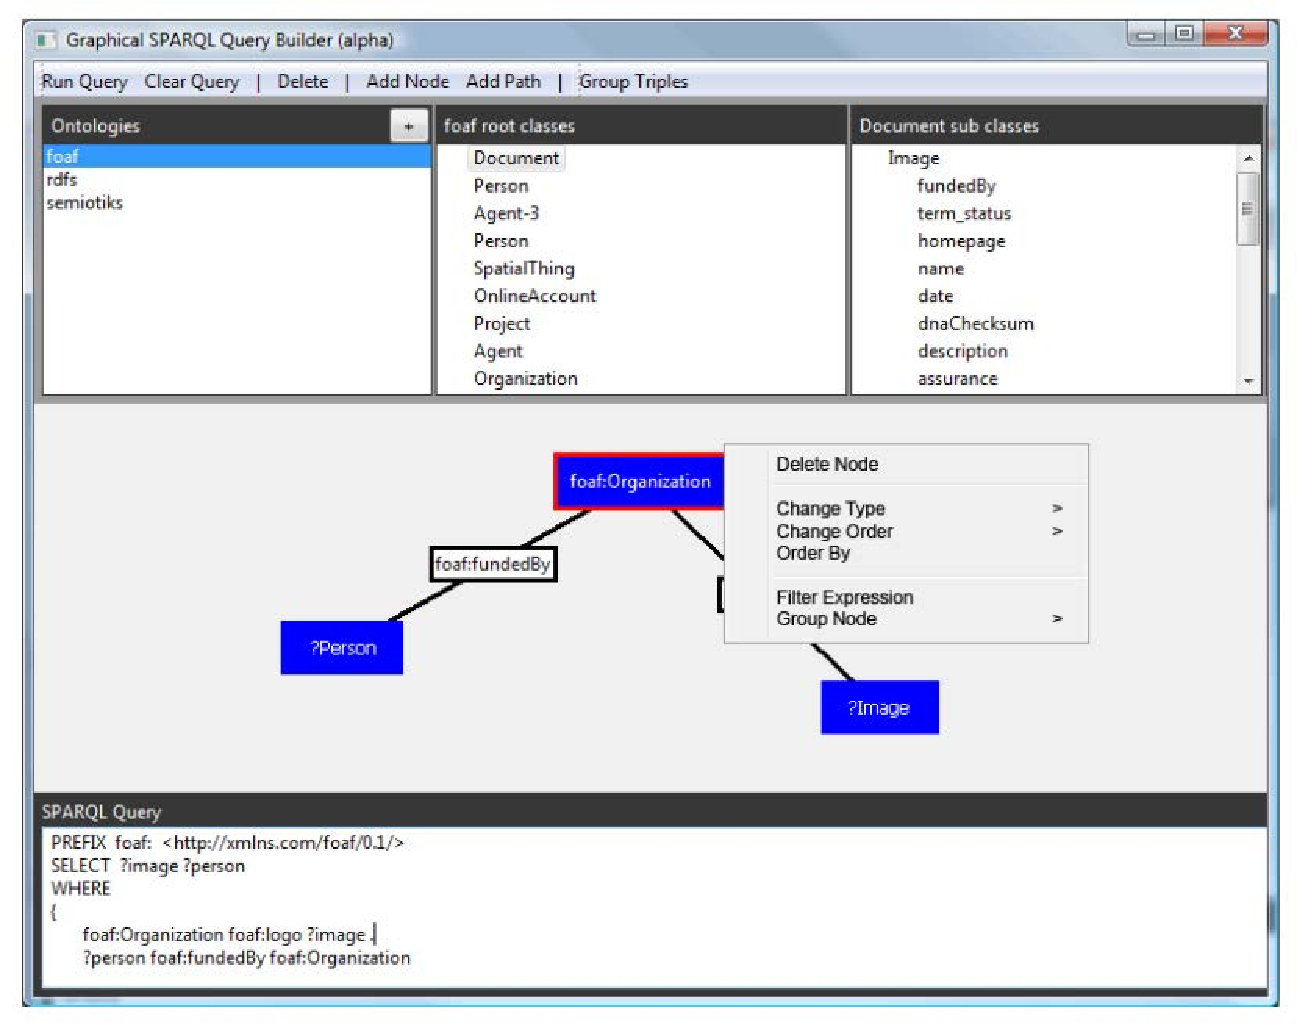
\includegraphics[width=.9\linewidth]{NitelightFigure1.pdf}
  \caption{An overview of the Nitelight user interface\cite{Nitelight}}
  \label{fig:NitelightUI}
\end{figure}
\\
Figure \ref{fig:NitelightUI} is an image of Nitelight in action. Nitelight is developed as a Java application and has some different tools to use. In the top it has basic commands such as running the query and adding new nodes. Below is the ontology browser, which can be used for the user to look through the different ontologies and what they consist of. Under the ontology browser is the node view, which is the main part of Nitelight. Here the nodes are set up in such a way that shows their relation to each other and this all results in the SPARQL query in the bottom. This text view is the result of the visual query and is read only.
\\\\
To elaborate on how the node view represents the finished query, use figure \ref{fig:NitelightBreakDown} for reference. Here it is shown that the query deals with three parts, the bound variable, the unbound variable and the literal predicate. The unbound variable points to the literal predicate, which then points to the bound variable. An example of this can also be seen in figure a, where a person (the bound variable) is funded by (the literal predicate) an organisation (unbound variable).

\begin{figure}[h]
    \centering
  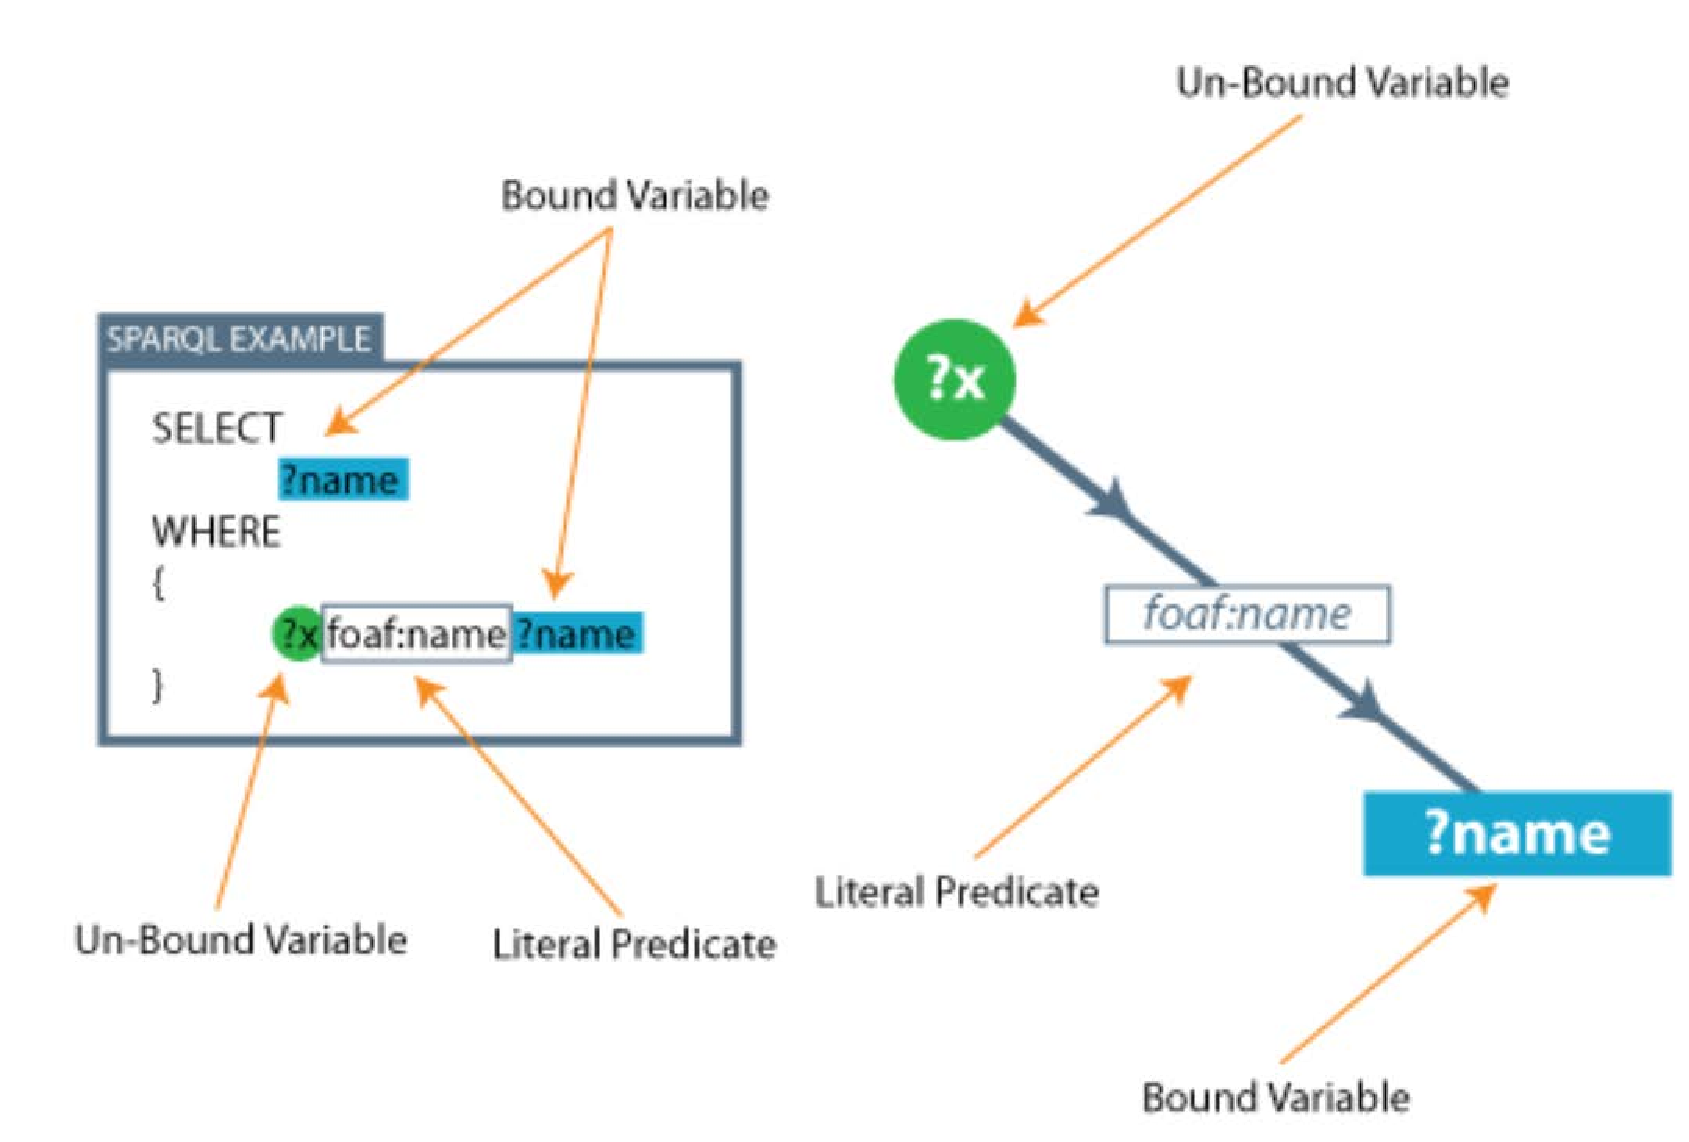
\includegraphics[width=.9\linewidth]{NitelightFigure2.pdf}
  \caption{Breaking down SPARQL queries to visualization\cite{Nitelight}}
  \label{fig:NitelightBreakDown}
\end{figure}

\subsection{QueryVOWL}
QueryVOWL is a visual query language to help users develop SPARQL queries\cite{QueryVOWL}, similarly to Nitelight. It is however developed as a webcomponent using HTML, CSS, JavaScript and SVG. It has three views, the main visual view, the sidebar for additional options and a result list containing the SPARQL query. The main view implements a drag and drop interface, which results in a completed SPARQL query without the need for the user to know perfect syntax. It can take any RDF dataset containing SPARQL endpoints.

\subsection{SPARQL-visualizer: A Communication Tool for Collaborative Ontology Engineering Processes}
This is a visualisation of the query result\cite{MadsHoltenSPARQL} and not the query itself. Therefore it could seem less relevant, however the way the graphical elements are implemented is something that can be used as inspiration. This leads to the library D3.js, a graphics library in JavaScript. The paper references (https://github.com/Rathachai/d3rdf) as a way to create a force layout of D3.js to visualize the expression "subject–predicate–object".



\section{Approach}
The solution will consist of a webcomponent, using JavaScript, that has two views for composing SPARQL queries, a textual and a visual. The visual view will be processed through SVG and should come in the form of a spring graph model layout. The user can interact with the visualisation through a drag and drop interface. The visualisation will then affect the textual view by writing the query in text. Likewise, will the visual view be affected by the textual view. Lastly, the visualisation has the option to be saved locally.

\section{Project goals}
The goals for this project are:
\begin{enumerate}
    \item To learn about RDF and SPARQL.
    \item To make a tool for visualising SPARQL queries.
    \item To make it easy to visualise and convert between a graphical and textual view of a SPARQL query.
\end{enumerate}

\section{Report structure}
{\color{red}missing\\}

\chapter{Method and Tools}
\label{chap:method-and-tools}

\section{Iterative development}
The iterative process is the development in different iterations each with their own well defined goal for what the purpose of set iteration is. This is referred to as sprints in some development processes. {\color{red}missing\\}

\subsection{Backlog}
The backlog has a list of all requirements that the software needs to be completed. This is essential for scoping iterations, tracking progress, and making sure that our software solution includes all the necessary tasks.

\section{Pair programming}
While both participants have experience with programming, it can be a good idea to incorporate pair programming. This has especially been helpful for this project as new libraries and concepts have been introduced. Pair programming helps ensure better code practices as the written code naturally comes into discussion. While useful, pair programming was not used at all times during development. As stated, pair programming has its advantages, but can be very time consuming and inefficient.

\section{Github and version control}
Throughout the project, github has been a vital part of development. Github is an online service for handling .git version control without having to write .git code. When developing in teams the need for version control is of considerable importance. This is due to the fact that it allows for each individual to work on two separate branches without any interference.
Furthermore, as this project deals in iterations, version control helps with pushing different working versions of the application. If a critical flaw is detected in new code, a rollback to a working version is always possible.


\chapter{Requirements}
\label{chap:requirements}

This chapter deals with defining and analysing of requirements for the project. To help determining the requirements, a list of use cases is created. The requirements are split into two categories: functional requirements and non-functional requirements. Using the two tools, MoSCoW  and FURPS , the requirements are then evaluated and prioritized.

\section{Use case}
Before determining the requirements, a list of use cases  is created to better understand what is essential for the user experience. This list can be seen in table \ref{tab:usecases} below.

\begin{table}[h]
\begin{tabularx}{\textwidth}{|l|l|X|X|}
\hline
\rowcolor[HTML]{9B9B9B}
ID   & Use case name      & Pre-Condition                                               & Post-Condition                                                    \\ \hline
\#01 & Add node           & Add node tool is selected                                   & After a successful creation, a node is added to the visualisation \\ \hline
\#02 & Draw arrow         & Draw line tool is selected, two nodes in visualisation      & A line is drawn between two nodes                                 \\\hline
\#03 & Delete nodes       & Nodes are selected                                          & The nodes are deleted from the visualisation                      \\\hline
\#04 & Delete arrows      & Arrows are selected                                         & The arrows are deleted from the visualisation                     \\\hline
\#05 & Write queries      & Text field is selected                                      & The text field is updated                                         \\\hline
\#06 & Save visualisation & Visualisation is not empty                                  & The visualisation has been saved locally                          \\\hline
\#07 & Edit node          & The edit tool is selected, a node is in the visualisation   & The node has been altered                                         \\\hline
\#08 & Edit arrow         & The edit tool is selected, an arrow is in the visualisation & The arrow has been altered    \\\hline   
\end{tabularx}
\label{tab:usecases}
\caption{Use cases for the program}
\end{table}

Each use case from table \ref{tab:usecases} is then expanded to include the possible scenarios in a separate table. An example of this is in \ref{tab:drawarrowusecase} which shows the extended version of the “Draw arrow” use case. By expanding the use case like this, the technical aspects of the use case can be described which can help in requirement elicitation and development.

\begin{table}[h]
\begin{tabularx}{\textwidth}{|l|l|X|}
\hline
\rowcolor[HTML]{9B9B9B}
Main Scenarios & Serial no. & Steps                                                                                          \\ \hline
Actors/Users   & \#01       & Click on two nodes                                                                             \\ \hline
               & \#02       & A popup occurs for arrow creation                                                              \\ \hline
               & \#03a      & Input name and press submit                                                                    \\ \hline
               & \#04a      & \begin{tabular}{@{}l@{}}An arrow is created\\ Close popup\end{tabular}                \\ \hline
               & \#03b      & Close popup                                                                                    \\ \hline
Extensions     & \#01       & \begin{tabular}{@{}l@{}}Nodes are already connected\\     Show error message\end{tabular} \\ \hline
               & \#03a      & \begin{tabular}{@{}l@{}}Name is not eligible\\    Show error message\end{tabular} \\ \hline                   
\end{tabularx}
\label{tab:drawarrowusecase}
\caption{Expanded use case for "\#02 Draw arrow"}
\end{table}

\section{Functional requirements}
Using the list of use cases, a set of functional requirements can be determined. The functional requirements are then prioritized using the MoSCoW method. This method deals with four different types of requirement prioritization: Must have, should have, could have, and will not have. The functional requirements can be seen in table \ref{tab:funcrequirements}.

\begin{table}[h]
\centering
\begin{tabular}{|l|l|l|}
\hline
\rowcolor[HTML]{9B9B9B}
ID  & Title                       & MoSCoW \\ \hline
\#01 & Node creation               & M      \\ \hline
\#02 & Arrow creation              & M      \\ \hline
\#03 & Writeable query             & M      \\ \hline
\#04 & Example of query            & C      \\ \hline
\#05 & Editable nodes              & S      \\ \hline
\#06 & Editable arrow              & S      \\ \hline
\#07 & Query and node highlighting & S      \\ \hline
\#08 & Visual and textual updating & M      \\ \hline
\#09 & Textual input parsing       & M      \\ \hline
\#10 & Parsing error handling      & S      \\ \hline
\#11 & Saving locally              & S      \\ \hline
\#12 & Uploading saves             & C      \\ \hline
\#13 & Multiple query types        & S      \\ \hline
\end{tabular}
\label{tab:funcrequirements}
\caption{Functional requirements}
\end{table}

Must have requirements are critical functionality. This means that without these, the program would be non-functional, or it would be impossible to implement other functionalities. An example of this is the node creation requirement. Without this functionality, there is not really a lot of program left. It would be impossible to work together with the textual view, saving the visualisation, add arrows, etc. Must have requirements are therefore often also reflected by the most important use cases.

\section{Non-functional requirements}
The non-functional requirements do not necessarily reflect the use cases but are requirements that influence the experience of the system. In this section, non-functional requirements are set through the process of a FURPS analysis. FURPS stands for: Functionality, Usability, Reliability, Performance, and Supportability. Functionality will be disregarded as this belongs to the functional requirements.

\subsection{Usability}
The target user for the application has no experience with RDF and SPARQL. This implies the application should focus on beginner level SPARQL and ease the user into writing queries. The application should be easy to figure out in the first couple of minutes. To help understand the concepts within SPARQL, the use of highlighting could be implemented into the system. This means that different attributes of the query could be highlighted consistently across the application making it easier to connect the visualisation to the written query. The user interface does not need to be visually pleasing, as the functionality is prime, but it should be consistent and therefore intuitive to use.

\subsection{Reliability}
The software needs to be working without any critical failures in the code. The application shall not store any user data, but it could be useful to cache the visualisation on updates, to help recoverability in case of shut-down failure. The application will not focus on loading times for different devices.

\subsection{Performance}
Once loaded, the application should run smoothly, preferably even on low end computers. There should not be any noticeable delay between actions. Actions should be done within 100 milliseconds of a user input, and if not, some sort of indication that the action is being processed should be shown.

\subsection{Supportability}
The application must be maintainable and open to future alterations. The application shall work as a web component and should therefore be easy to add to a webpage. The application will not be expected to support other devices than PC’s.

\chapter{First iteration}
\label{chap:first-iteration}
In this chapter the first iteration is discussed. The first iteration included the initial analysis and design in which two different design models will be shown: The first theoretical design and the actual design. Afterwards the fruition of the design will be discussed in the implementation segment. Lastly an evaluation of the iteration, which deals with the issues of the current application and how to improve it in the next iteration.

\section{Analysis and Design}
\subsection{The SPARQL object}
As SPARQL is the main essence of the project, the SPARQL class will be the primary focus of the design. The principle of the SPARQL class is to implement essential functionality of a SPARQL query. This means that it should be possible to take a given SPARQL query and break it down into this class form. With this class, SPARQL objects can be created, which can be sent as a common ground between the visual and the textual parsers. A simplistic overview of the relation can be seen in \ref{fig:sparql-interaction} below.
\begin{figure}[h]
    \centering
    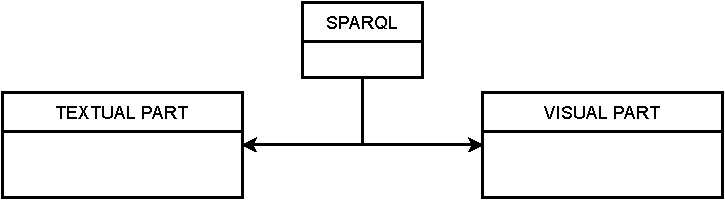
\includegraphics[width=1\textwidth]{figures/sparql-interaction.pdf}
    \caption{Simplistic overview of the relationship between the parsers and the SPARQL class}
    \label{fig:sparql-interaction}
\end{figure}

\subsection{From Query to class}
As the focus of the project is to implement simple queries into the system, select queries have been the heart of the SPARQL class.  By using the SPARQL query in figure \ref{fig:sparql-example}, the following class diagram is created, figure \ref{fig:SPARQL-Triple-class}

\begin{figure}[H]
    \centering
    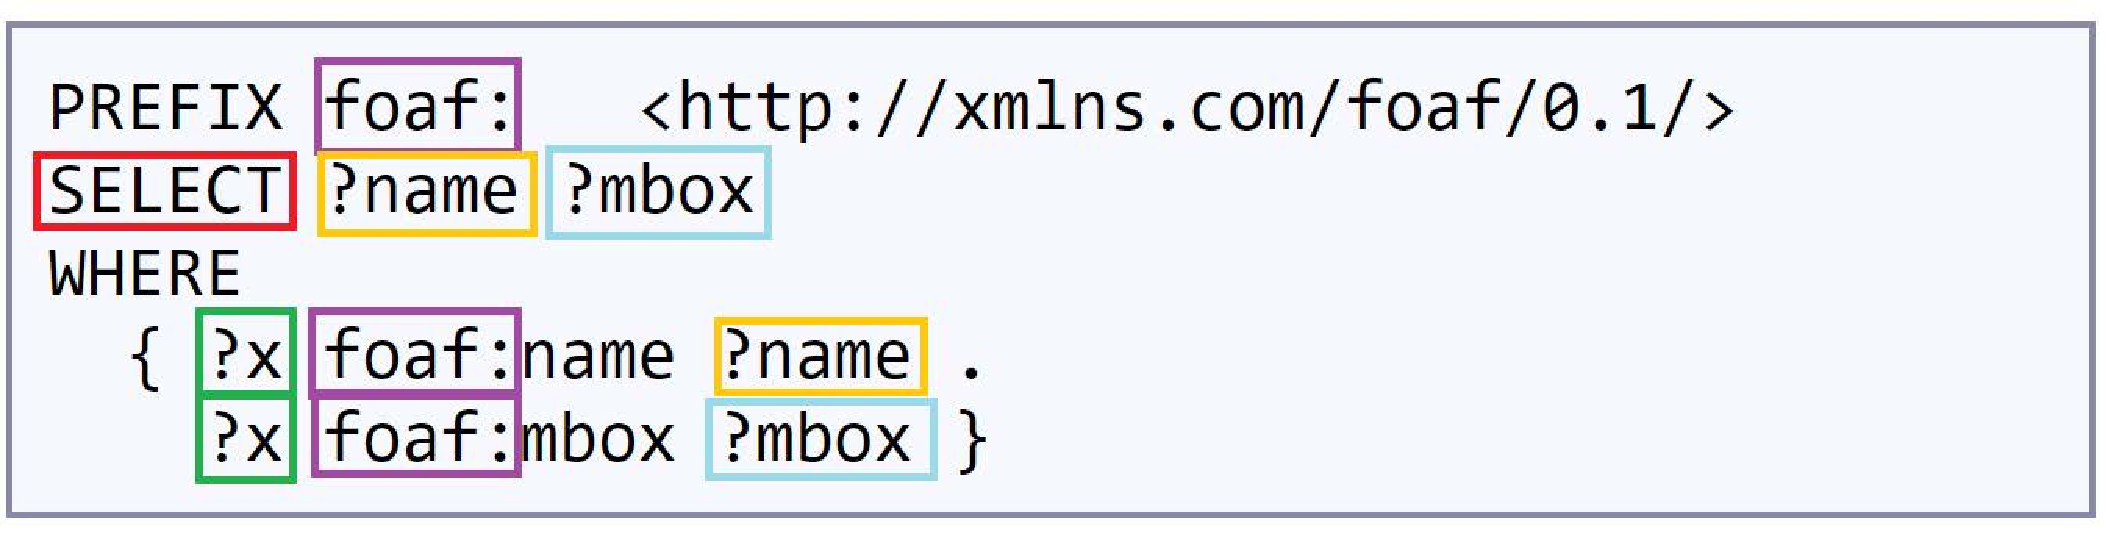
\includegraphics[width=1\textwidth]{figures/sparql-example.pdf}
    \caption{SPARQL query with highlights}
    \label{fig:sparql-example}
\end{figure}

\begin{figure}[H]
    \centering
    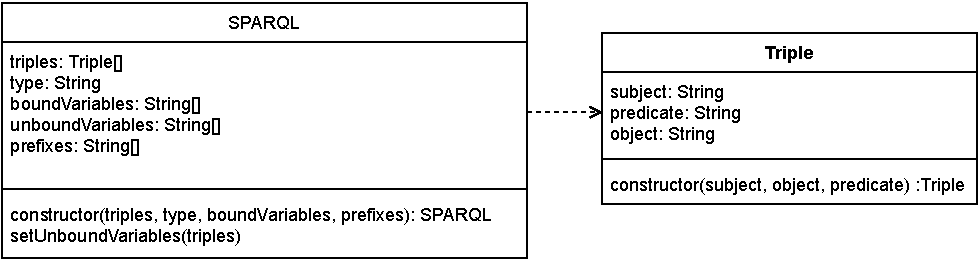
\includegraphics[width=1\textwidth]{figures/SPARQL-Triple-class.pdf}
    \caption{Class diagram for SPARQL}
    \label{fig:SPARQL-Triple-class}
\end{figure}

As it can be seen in figure \ref{fig:SPARQL-Triple-class}, a couple of different variables are defined for the SPARQL class. First is the Triple array. This array contains all the “triples” in the query. Triples are normally reserved for RDF, but the principle can be used in SPARQL as well, in which they are called graph patterns. An example of a graph pattern in a SPARQL query could be “?x foaf:name ?name”, which can be found in the WHERE section of the query, see figure \ref{fig:sparql-example}. A triple therefore consists of three strings: a subject, a predicate, and an object. Next is the type of the query, which can be SELECT, CONSTRUCT, DESCRIBE, and ASK, but for the current version of the program only SELECT is implemented. Bound and unbound variables can be found in the triples as well, but the difference is that bound variables are included in the top of the query next to the type. Regarding figure \ref{fig:sparql-example}, the bound variables are the variables the user wants to select. Lastly the prefixes are stored in an array.

\subsection{Textual parser}
 When it comes to the textual parser the goal of the first iteration is familiarising ourselves with the concepts of a parser. The entire idea of a parser is taking some text and figuring out patterns to allow for the software to return some data based on what is written, in our case we want to be able to write a SPARQL query and convert it to the SPARQL object we have created so we can share the information between the visual and textual parts. To keep this as simple as possible we wanted to do this with already known easy to under technologies. The first challenge is to figure out how we get text to something readable for the software, then we have to figure how are we going to match the text to a pattern we expect to see and lastly how are we going to convert from the textual pattern to an object and from an object to the textual pattern
 
\subsection{First design}
Based on the requirements in the previous chapter and the class diagram in figure \ref{fig:SPARQL-Triple-class}, a complete system design is created, see figure \ref{fig:initial-design}. The design is primarily based on the must have requirements. Starting on the side of the visual part, a visual handler and a visual parser has been added. The job of the visual handler is to control the visualisation. This means it will handle requirements such as node creation and arrow creation. The visual handler has a two-way connection with the visual parser. The visual parser gets the visualisation from the visual handler by a call of the “getVisualisation” method. This returns a set of SVG elements, which the visual parser shall convert to a SPARQL object and send to the textual parser. The conversion between SVG elements and SPARQL object shall be done by taking any textual attributes in the visualisation and append them as the triples of the SPARQL object. The textual parser shall then take the SPARQL object and convert it to one string for the textual handler, which will update the text field on the page. The text field will be for query writing and is correlated to the requirement of the similar name: Writable query. This entire process of converting it from a visualisation to a SPARQL object, and then a text string shall be reversed so a two-way relationship can occur. This corresponds to the functional requirement “Visual and textual updating”.

\begin{figure}[H]
    \centering
    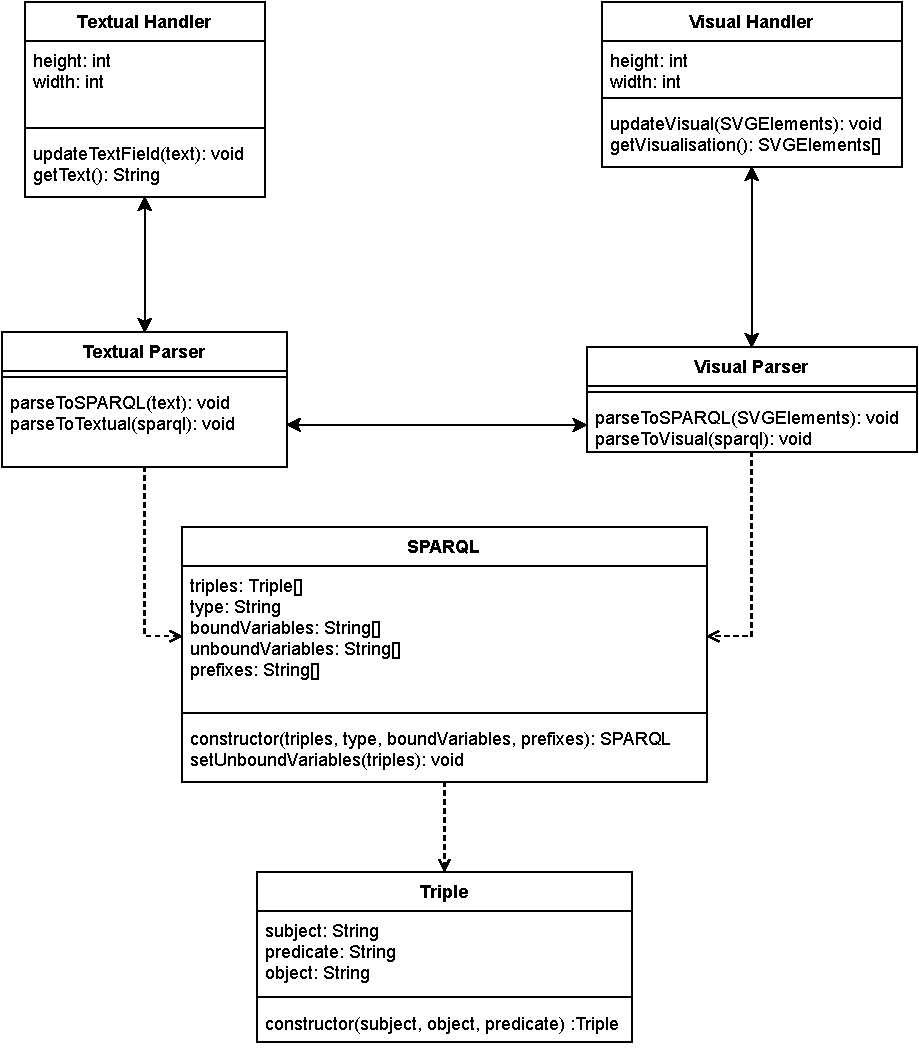
\includegraphics[width=1\textwidth]{figures/initial_design.pdf}
    \caption{The first design}
    \label{fig:initial-design}
\end{figure}

\subsection{Actual design}
During implementation, some complications arose with the initial design. The main issue was the conversion from visual handler to visual parser. In the first design, an array of SVG elements was sent to the visual parser. This was troublesome as it is difficult and very code heavy to extract the text attributes from the array and figure out where they belong. Therefore, a new design was created, figure \ref{fig:first-design}, in which the two classes Arrow and Node have been added. These classes both contain the relevant SVG for creating their visualisation, and act as a datatype which can be transferred between the visual handler and the visual parser. As the arrow class represents a graph pattern, a conversion can be made simply by sending the array of arrows in the visualisation.

\begin{figure}[H]
    \centering
    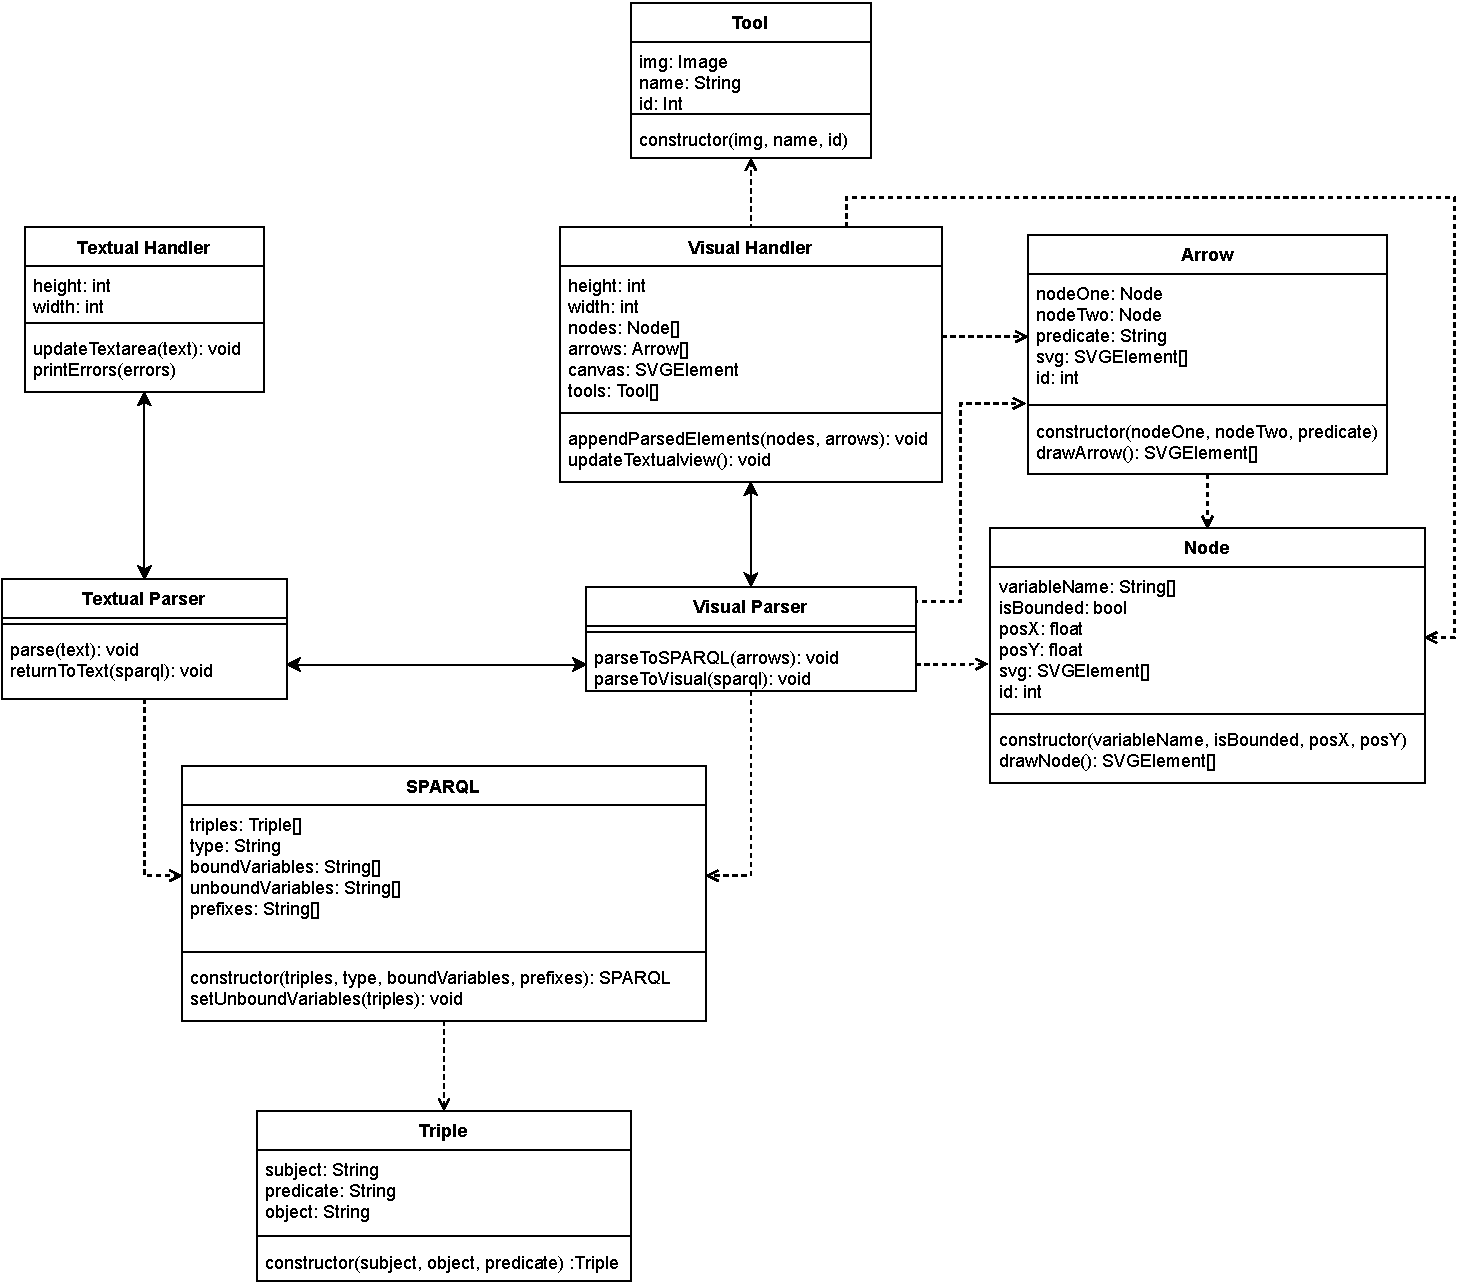
\includegraphics[angle=90,origin=c,width=1.3\textwidth]{figures/1st_iteration_design.pdf}
    \caption{The actual design}
    \label{fig:first-design}
\end{figure}

\subsection{SPARQL visualised}
In the requirements section it is stated that the visualisation shall be made from nodes and arrows, but first the nodes and arrows must be specified to know what they contain and what they resemble. As mentioned earlier in the chapter, SPARQL utilises sets of triple patterns, a graph pattern, to construct queries. These triple patterns mimic the RDF triple pattern of a subject, predicate, and object, and can be substituted for variables in the queries.

\bigskip
Looking at the SPARQL query in figure \ref{fig:sparql-example}, the most important parts of the query have been highlighted. The purple boxes highlight a prefix, in this case foaf, red highlights the type of query, select, yellow and blue boxes represent variables, and green boxes for the subject. All the highlights are however not necessarily node worthy in the visualisation. As an example, the type of query is not needed as a node but perhaps an option on the side.

\bigskip
A couple of suggested UI designs, which can lead to multiple combinations, can be seen in appendix {\color{red}x.x}. These designs are directly correlated with figure \ref{fig:sparql-example}, meaning the colours are the same. This relates to the requirement “Query and node highlighting”. The requirement “Select different queries” has two options. Either it shall be a node connected to the bound variables or a selection outside of the canvas. This is doable as the possibilities are limited to 4: Select, Construct, Ask, and Describe. The advantage of using the node form is that it is easily visible which variables are the bound variables. However, there is also room for confusion both in code and visually. New users might think that the type node is a part of a triple. Code wise, it is important to distinguish between the different types of nodes, as it is important not to convert it to a triple. As it can be seen in figure \ref{fig:chosen-ui}, which is the final choice of visualisation, the choice fell on the type selection disconnected from the canvas. This was because it should already be possible to see the bounded variables by their colour, while the disconnect avoids confusion.

For the arrows between the nodes, the selection came between an arrow with a name above or yet another node with a name. The second solution did however not make any sense and was more confusing than helpful. It was therefore decided to just use arrows as it can be seen in figure \ref{fig:chosen-ui}.

\begin{figure}[H]
    \centering
    \includesvg[width=1\linewidth]{figures/UI_idea_1.svg}
    \caption{The chosen UI for the visualisation}
    \label{fig:chosen-ui}
\end{figure}


\section{Implementation}
\subsection{Visual implementation}
For the first iteration, the visual implementation had to have the following features:
\begin{itemize}
    \item A canvas with node creation and manipulation.
    \item A two-way conversion between SPARQL objects and the visualisation.
\end{itemize}
This led to the following solution, figure \ref{fig:visual-ui-first}.

\begin{figure}[H]
    \centering
    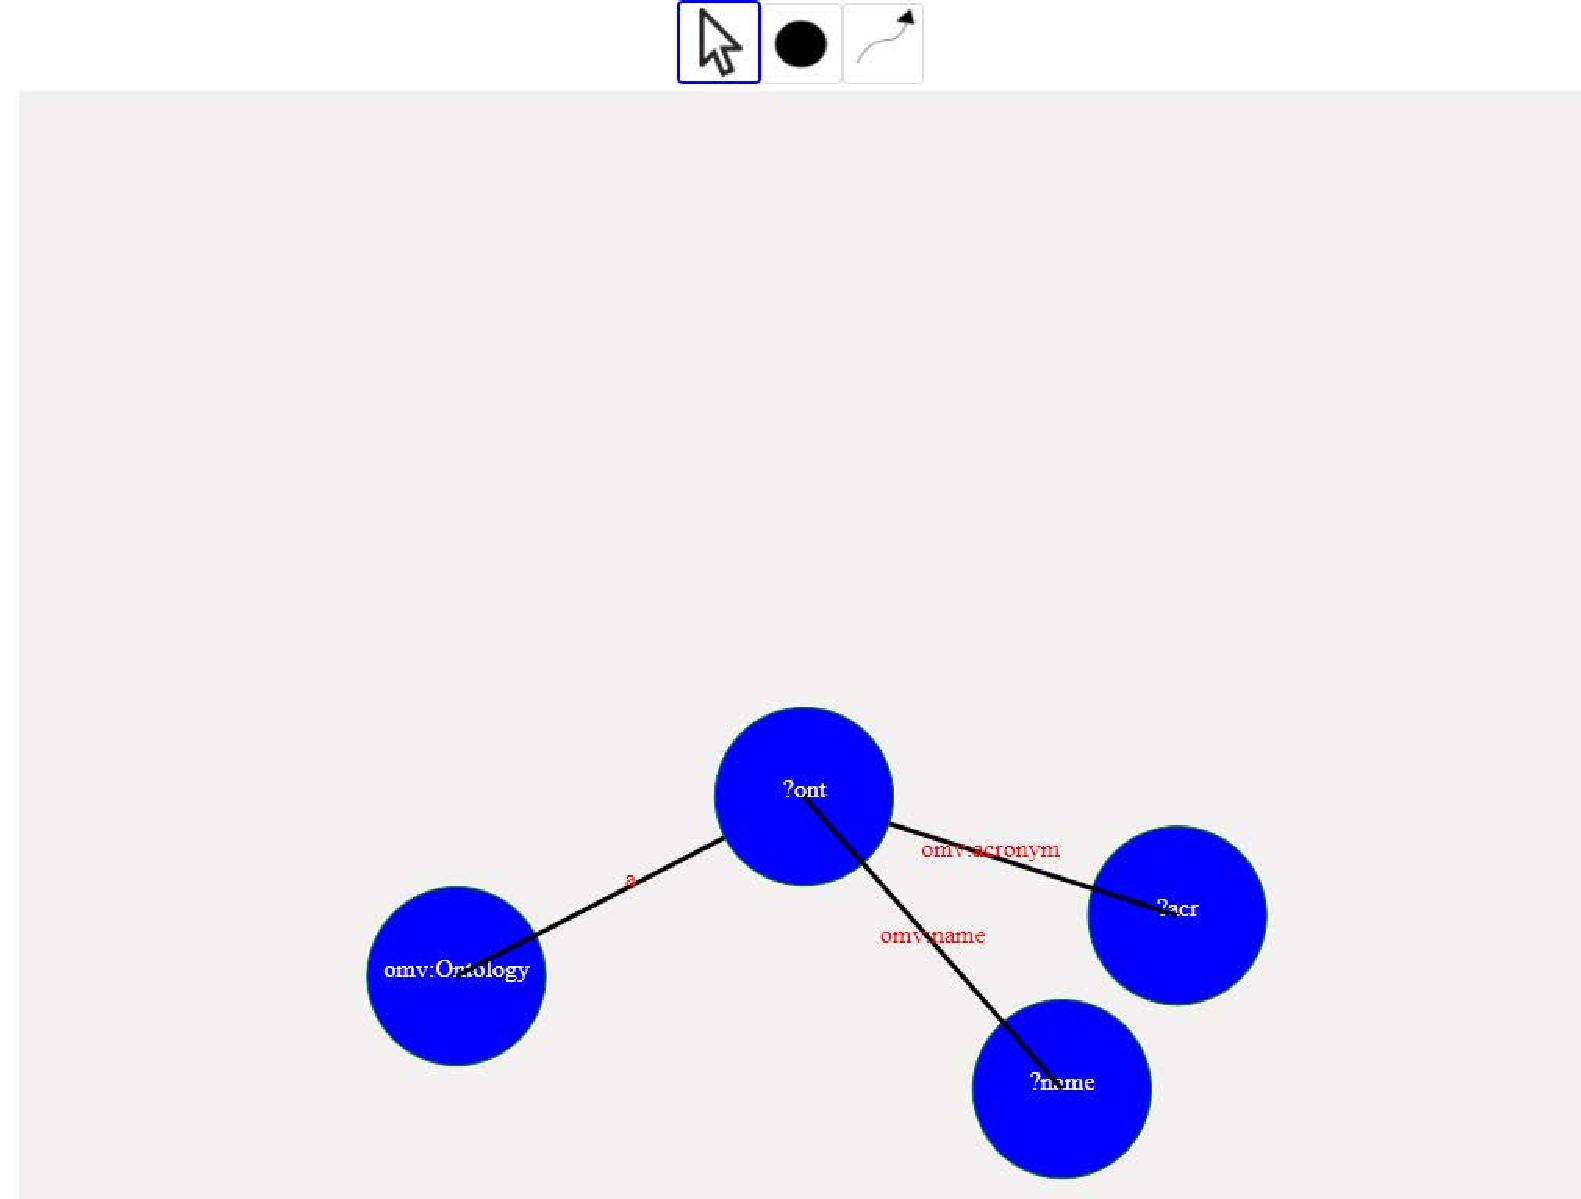
\includegraphics[width=1\linewidth]{figures/visual-ui-first.pdf}
    \caption{Snippet of the visual part of the program.}
    \label{fig:visual-ui-first}
\end{figure}
The figure above shows the visualisation of a simple SPARQL query. As discussed in the design segment, each node represents a variable, subjects and objects, and the lines between are the predicates of the graph pattern. Above the canvas, which is the grey area surrounding the nodes, three different tools are shown. The first tool is for selecting nodes and lines, which can then be deleted from the visualisation. The second tool is for node creation and the third is for line creation. Figure \ref{fig:visual-arrow-node} shows the popups created from the last two tools.

\begin{figure}[H]
    \centering
    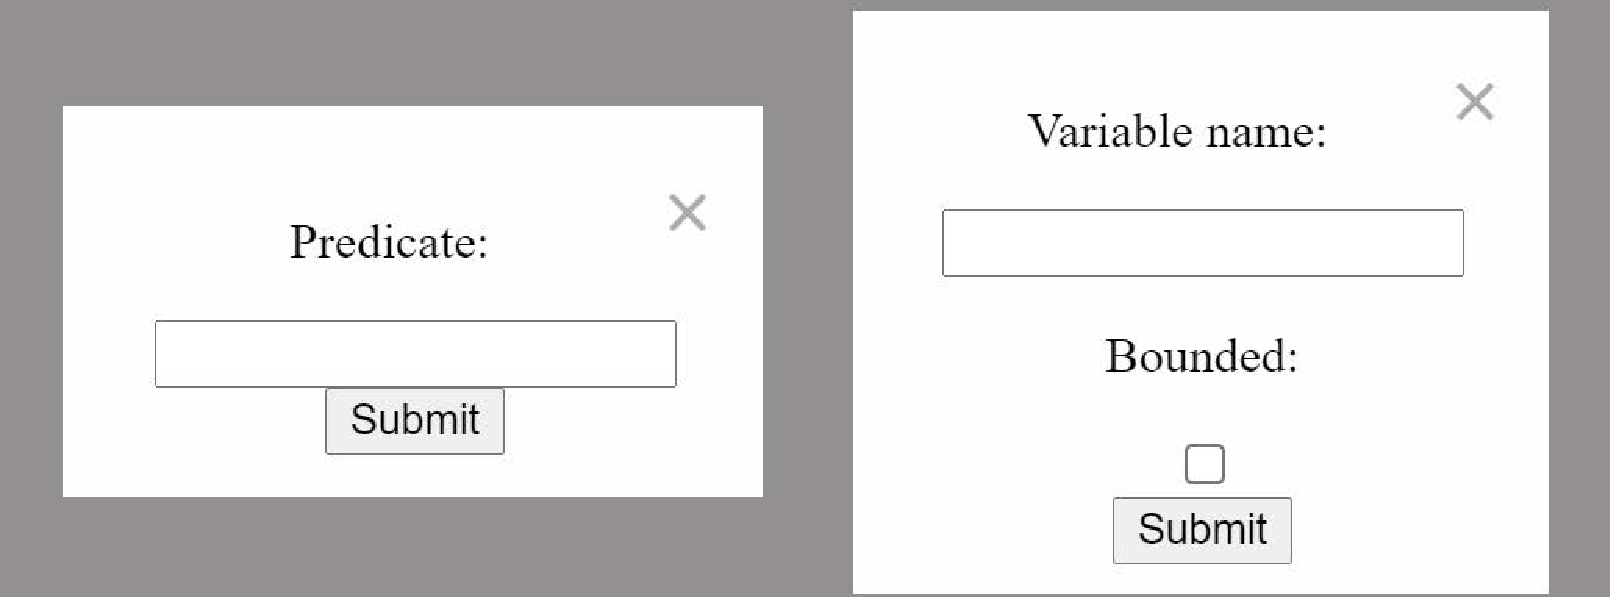
\includegraphics[width=1\linewidth]{figures/visual-arrow-node.pdf}
    \caption{Left is the line tool popup, right is the node creation tool popup.}
    \label{fig:visual-arrow-node}
\end{figure}

\subsection{Force directed spring graph layout}
While it is difficult to see in figure \ref{fig:visual-arrow-node}, the visualisation is affected by forces which have an impact on node positions and the lengths of the lines. This helps the visualisation commit to a spring graph layout without overlaps in nodes. This was implemented using the following algorithm, figure \ref{fig:algo}:
\begin{figure}[H]
    \centering
    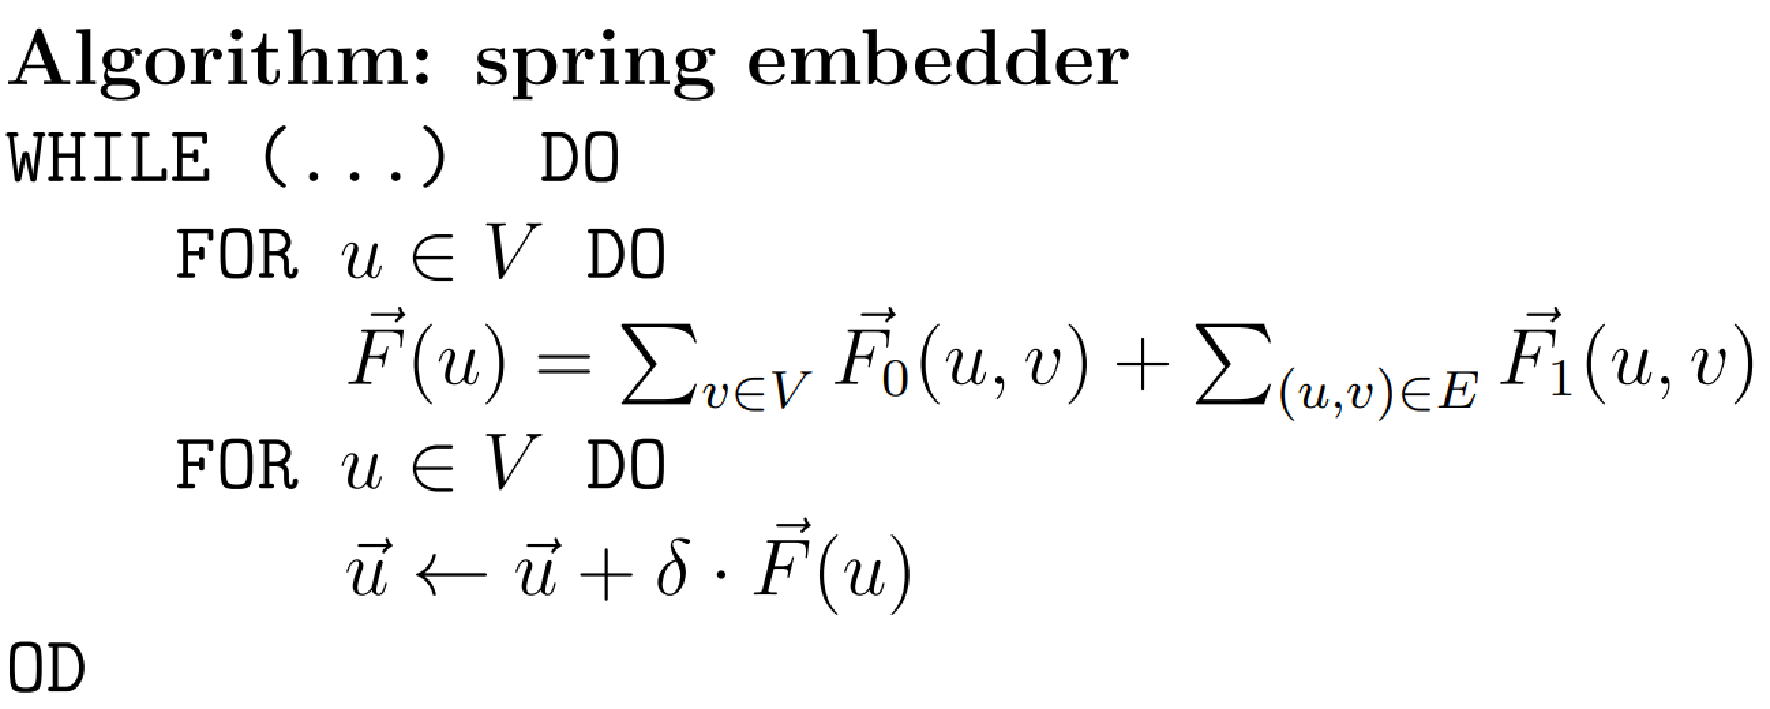
\includegraphics[width=1\linewidth]{figures/algo.pdf}
    \caption{Algorithm for a spring graph layout from Praktikum Algorithmen-Entwurf}
    \label{fig:algo}
\end{figure}
The algorithm takes a given graph with the vertices V, nodes, and edges E, arrows. Then for each vertex two combined forces are applied. The first force acts as a repulsive force between the vertices and will separate the vertices from each other. The second force is the force of the edges. The job of an edge is to hold two vertices together and therefore the force is counteracting the initial repulsive force of the vertices. A second for loop then applies the force to the position vectors of the vertices. This algorithm is meant to run while the combined forces are not equal to zero. However, zero can be a difficult value to hit exactly and the algorithm can therefore be run in several iterations or until the combined force is within a certain threshold. In this implementation, the algorithm runs until the force is within the range {-1,1}.

\subsection{Textual implementation}
The parser in the first iteration worked based on “if statements” and simply looking if the next character in the text was the character that was expected and if not print an error citing where and what the error was. This was a decent enough approach to get something that works but it was not great for maintaining as the potential for bugs was very high since any tiny error on our end would break the entire system or if the user used slightly different spacing than what was expected it could potentially also break fx. a double space instead of a single space. The use of a series of if statements is also very inefficient which for our relatively small scale and beginner friendly prototype is not the biggest concern as it does not scale well. Another issue with doing it this way is that implementing a new type or other new features would require one to check everywhere to make sure nothing broke and not only the part that was changed/added meaning that the code could not really be reused for multiple different types/inputs\\
To look at a code example of how this long list of if-statements worked see figure \ref{fig:textual-parser}.
\begin{figure}[H]
    \centering
    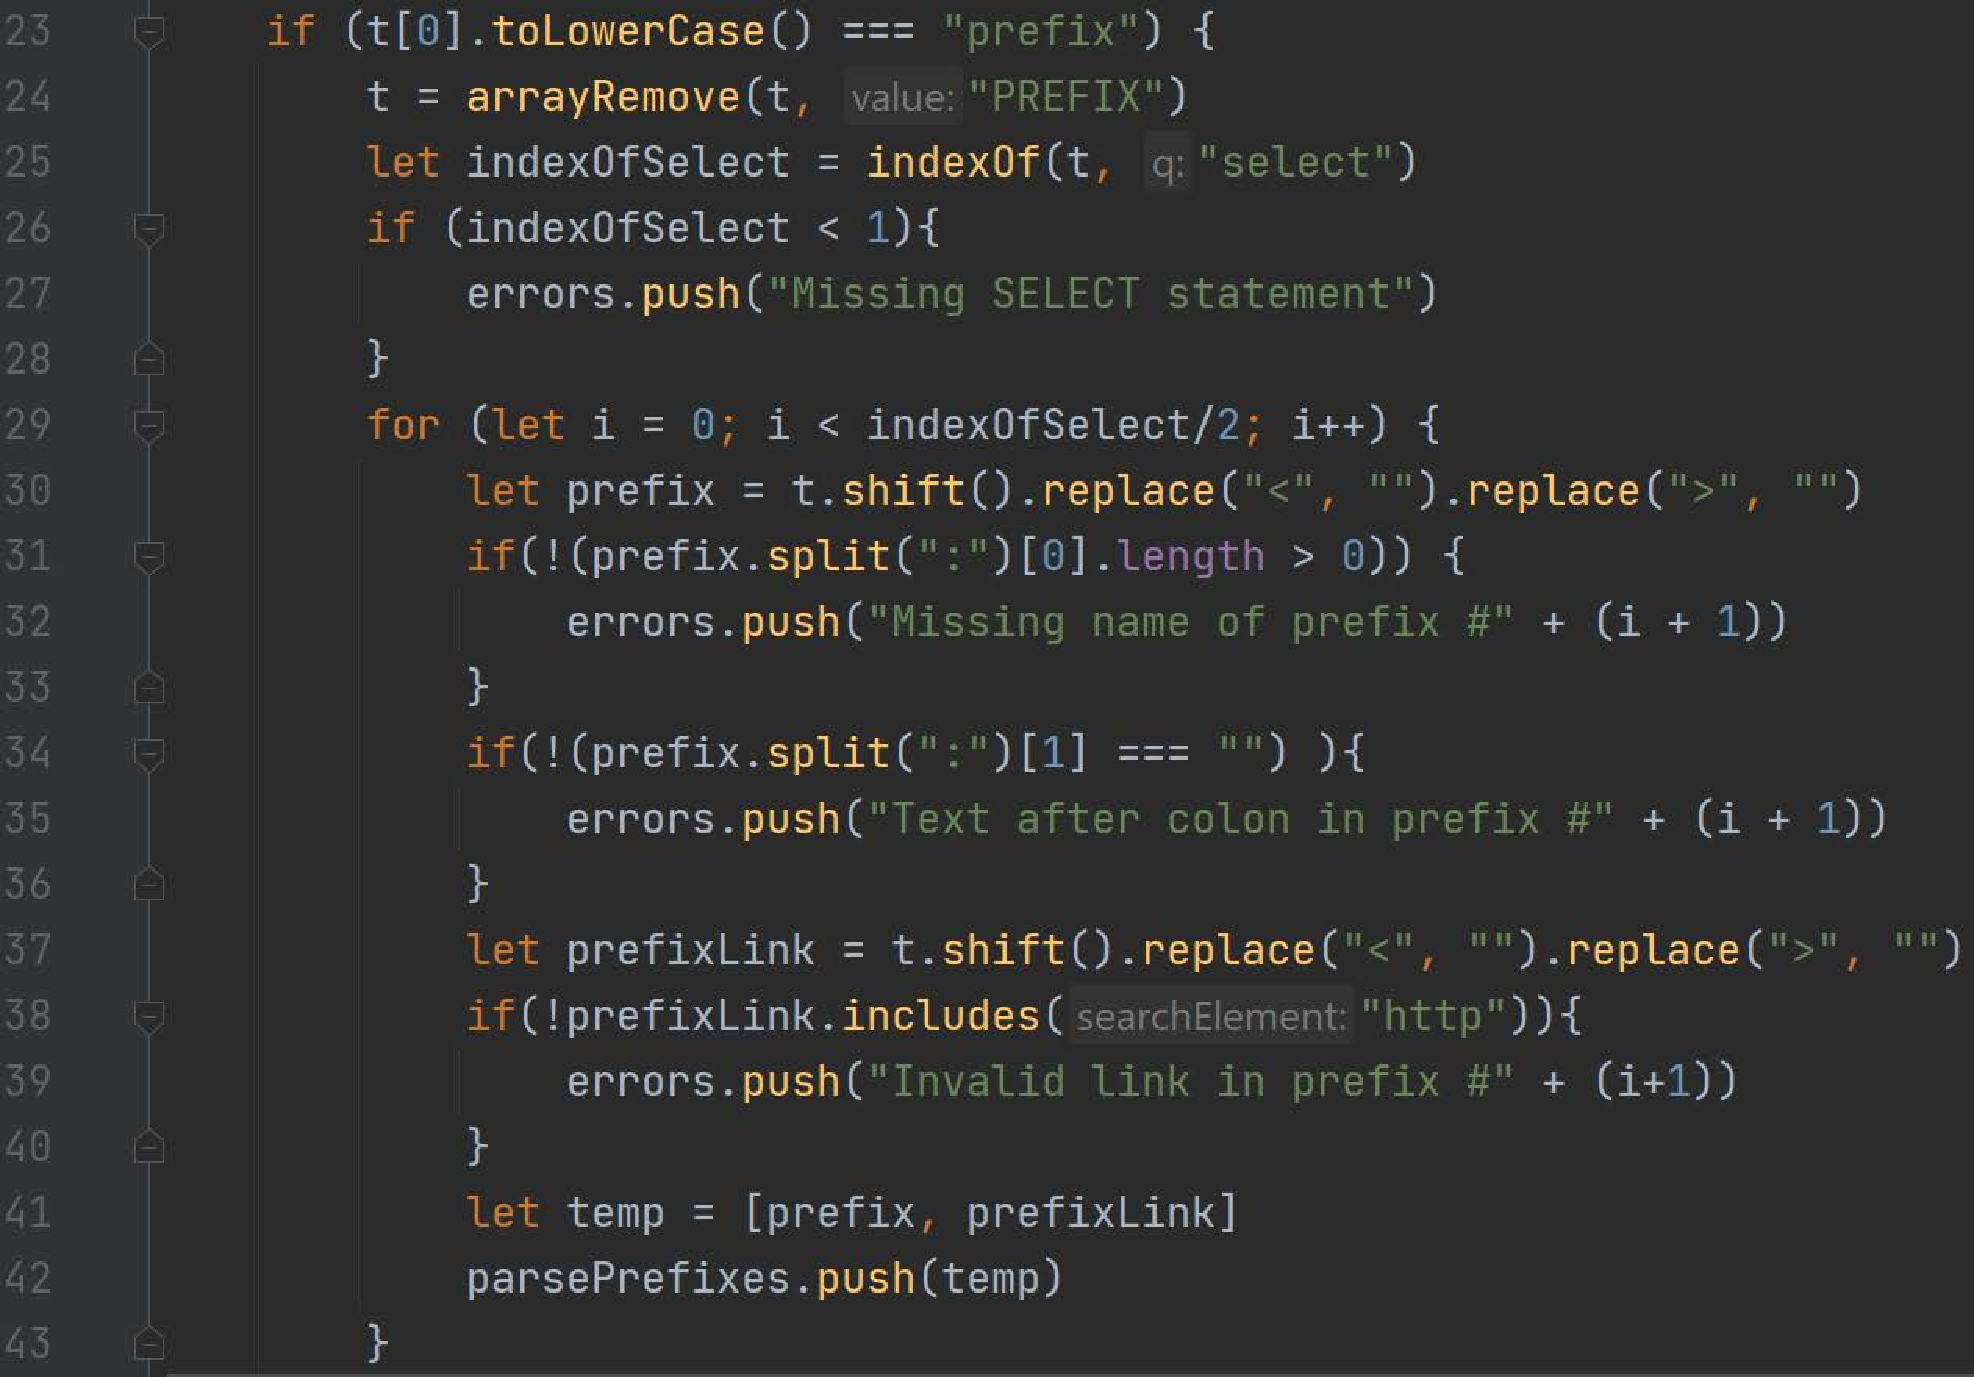
\includegraphics[width=1\linewidth]{figures/textual-code-first.pdf}
    \caption{Code example from the textual parser}
    \label{fig:textual-parser}
\end{figure}
The first step was to look at if the first character was the word “prefix” this was done to determine if the user had any prefixes in their query so we could handle these first. The next step was to remove all the instances of the word prefix as we do not care about those anymore, then we get the index of the “select” keyword meaning when the user’s last prefix is done. A quick check to make sure the word select was found or else we could make an error to say that it is missing. The next step is to run through each prefix and get the name and link so we can add them to the SPARQL object in the end. To do this we decided on first removing the angular brackets as these would just potentially mess with the names, then we checked is there a name of the prefix included and if not create an error saying that there is no name in this prefix, then we had to ensure there was no text after the colon in the prefix as a prefix is defined as a name ending with a colon. The last step was to make sure that the link included was valid and then push it to the prefixes array.

\section{Evaluation}
The first iteration had lived up to the given requirements, but the solution was subpar. As the whole visualisation was created only using vanilla JS and SVG, algorithms connected to graph theory had to be entirely implemented by the group. This meant that while functional, the look of the program became harsh looking. The force directed graphing moved the nodes into the right positions, but the translation of the nodes was not smooth. The nodes and lines were overlapping depending on which element had last been added, and while this is fixable, the solution will probably lead to a less than practical approach.

The textual parser was also not without its flaws, the biggest issue we ran into was the problem of code extension, the parser was built so specific to handle one case that any extension of the code would require an almost full rewrite. The parser also struggled with error handling as this was hand made meaning that any error we did not think of would break the system there was no automatic “unexpected character” or anything similar. The last three majors were all due to the way we decided to implement the checks for whether a pattern matched, the implementation choice of using if-statements seemed like a good idea at the start since it was a known and simple technology, later it would prove to cause issues with performance, maintainability, and readability. The performance was due to having to check each word whether it matches a long series of patterns, the maintainability issues was due to having to decipher these long pattern matches made it almost impossible to edit without breaking something elsewhere. The issue of readability matches closely with the issues of maintainability since the long pattern matches were almost impossible to read and understand even to the point where it was hard for the others in the group to understand what was going on.

\chapter{Second iteration}
\label{chap:second-iteration}
The second iteration was all about improving the issues outlined in the evaluation of the first iteration, this is also the final iteration in the project and leads to a complete product by the end. This chapter will include an analysis of the problems from the first iteration for the textual and visual elements, a description of how the design changed trying to solve these issues, how we implemented the changes and lastly an evaluation and what could be improved and what worked.
\section{Analysis and Design}
\label{chap:second-analysis}

\subsection{Textual analysis}
The biggest change in the second iteration is going from a hand-made/native solution to the use of external libraries. This change was done on the basis of some of the issues we ran into during the first iteration. For the textual element this includes the following table of issues:
% Please add the following required packages to your document preamble:
% \usepackage[table,xcdraw]{xcolor}
% If you use beamer only pass "xcolor=table" option, i.e. \documentclass[xcolor=table]{beamer}
\begin{table}[H]
\begin{tabularx}{\textwidth}{|l|l|X|}
\hline
\rowcolor[HTML]{9B9B9B} 
ID   & Name               & Description                                                                                                                                                                                                \\ \hline
\#01 & Extending the code & The issue with code extension was due to the fact that the entire code was written to handle one specific type of query and not a multitude of different queries (see more in first iteration chapter)     \\ \hline
\#02 & Error handling     & The error handling was not great as it was all custom written, meaning if there was an unforeseen error there would be no help for the user. This leads to frustration when you are a new user.            \\ \hline
\#03 & Code performance   & As mentioned in the evaluation of the first iteration there were issues with the performance of the code. The code was a collection of if-statements, which is quite inefficient for handling big queries. \\ \hline
\#04 & Maintainability    & Any bug in the code was close to impossible to identify as the code was written as long conditions for if-statements meaning that it could be hard to gage what is going on.                               \\ \hline
\#05 & Readability        & The readability was very poor. This meant it was difficult to for others to understand and potentially find bugs                                                                                           \\ \hline
\end{tabularx}
\label{tab:parser-issues}
\caption{The issues with the parser from the previous iteration}
\end{table}

To solve these issues, the group decided on the use of an external parser as it was an insurmountable task to solve all these issues with the current way of development. To help decide on a specific parser, the group made some evaluation criteria for how to rank the parsers from one another. This was helpful due to the lack of knowledge regarding the subject and no specific parser came to mind. The evaluation criteria are as follows:

% Please add the following required packages to your document preamble:
% \usepackage[table,xcdraw]{xcolor}
% If you use beamer only pass "xcolor=table" option, i.e. \documentclass[xcolor=table]{beamer}
\begin{table}[H]
\begin{tabularx}{\textwidth}{|l|l|X|}
\hline
\rowcolor[HTML]{9B9B9B} 
ID   & Name           & Description                                                                                                                                                                                                                                                                                                                                                                                                                                                                                                                                                                         \\ \hline
\#01 & Error handling & \begin{tabular}[c]{@{}X@{}}The number one priority for the parser was to have great error handling as our software is targeted towards new users. To be able to see where they are going wrong is the single most important thing.\\ To give a metric on how to evaluate error handling we made a list of error handling features it should include:\\ 
\begin{minipage}[t]{0.65\textwidth}
    \begin{itemize}
    \item Knowing what the errors, including the expected result ie. Found “x” expected “y”
    \item   Knowing where the error is, to allow for line number and highlighting ie. Error on line 32, character 5\\
    \end{itemize}
  \end{minipage}    
    \end{tabular} \\ 
    \hline
\#02 & Ease of use    & \begin{tabular}[c]{@{}X@{}}As said the group has little to no experience working with a parser or similar technology so ease of use would rank highly as we have limited time to learn an entire new technology and did not think it was a valuable use of our time.\\ The metrics for the ease of use are as follows:      
\begin{minipage}[t]{0.65\textwidth}
    \begin{itemize}
    \item Parse generation means that we do not have to write code but can just write rules.
    \item   An online editor or examples to play around with when learning the parser\\
    \end{itemize}
  \end{minipage}    
    \end{tabular} \\ 
    \hline
\#03 & Performance    & The last evaluation criteria is the performance of the parser. The reason for this being the least important is due to the target demographic mainly using our software as a stepping stone. This means they will most likely not use it for bigger projects as that is not the intended use and there are better solutions for that. Performance can be a more specific metric than the other criterias, as you can put a number deciding fast it should be able to process a worst-case scenario.                                                                                 \\ \hline
\end{tabularx}
\label{tab:parser-issues}
\caption{Evaluation criteria for the textual parser}
\end{table}

To gather a list of potential parsers to use, the group found the following website: https://chevrotain.io/performance/.This website contains benchmarks and comparisons for 11 different parsers. These comparisons are done on “an input sample of an around 1000 lines JSON file”\cite{parsePerformance}. As this is a benchmark test it is only ranked in terms of performance, see below for full rankings. The group is aware of the potential bias in these rankings as the site ranks the parser the site is built around.  This does not play a big role as it was mostly used to gather a list of parsers and not as much the performance aspect of each parser.
To rank the other two categories, an analysis was made as seen in the table below:

% Please add the following required packages to your document preamble:
% \usepackage[table,xcdraw]{xcolor}
% If you use beamer only pass "xcolor=table" option, i.e. \documentclass[xcolor=table]{beamer}

\begin{table}[H]
\begin{tabularx}{\textwidth}{|l|l|X|X|}
\hline
\rowcolor[HTML]{9B9B9B} 
ID & Name       & Error handling                                                                                                                                  & Ease of use                                                                                                                                  \\ \hline
01 & Chevrotain\cite{ChevrotainGithub} & Good error handling with some decent highlighting of where things go wrong. Has all the features we are looking for in terms of error handling. & No parse generation, meaning we have to write the code for the parser itself which is a big hassle. A good online editor nothing too special \\ \hline
02 & ANTLR4\cite{ANTLRGithub}     & Requires some work to get the error handling we want                                                                                            & No online editor and quite challenging grammar structure                                                                                     \\ \hline
03 & Parsimmon\cite{ParsimmonGithub}  & Requires a bit of work to get a readable error text, but includes both features                                                                 & No online editor, and no parse generation                                                                                                    \\ \hline
04 & PEG.js\cite{PEGJSGithub}     & Really good error handling provides everything we want                                                                                          & A great online editor and easy to understand and play with grammar                                                                           \\ \hline
\end{tabularx}
\caption{}
\label{}
\end{table}

The rest of the entries were lacking behind PEG.js in all three categories and we therefore did not find it necessary to include them in this table. In the end the decision to go with PEG.js was made as the parser of choice due to it having the best combination of error handling and ease of use, and even with the quite low ranking in performance it is still more than fast enough to process the data we need for this solution. 



\subsection{Visual analysis}
To fix the issues regarding the visualization, which was outlined in the evaluation of the 1st iteration, the decision landed on using an external library for the visualisation. The chosen library was D3.js. D3.js is a visualisation library that helps creating visualisations in fewer and, and probably more efficient, lines of code\cite{useD3}.  D3.js is also a library that the group has come across several times in resolving SVG related issues. D3.js is one of the most popular visualisation tools for JavaScript, and this leads to a great amount of documentation in the form of tutorials, video guides, premade examples, and Q\&As. The huge amount of documentation did however turn out to cause some confusion at times as D3.js comes in different versions with previous version methods becoming obsolete and faced out. It was therefore of huge importance to ensure the right documentation version was found when working with D3. D3 is also very modular, and the necessary modules can be imported, setting up for shorter load times.
A big factor in switching to a library such as d3.js, was the implemented force layout in iteration one. As mentioned in the evaluation, the force implementation was rough looking and took time to settle. In d3.js, force is a module which can be imported, and a force directed graph is quite common to find in d3 documentation\cite{forcedirectedD3}.

\subsection{Design}
The use of external libraries allowed us to simplify the design greatly, as we could remove some of the external classes and simplify the methods in the kept classes.

\begin{figure}[H]
    \centering
    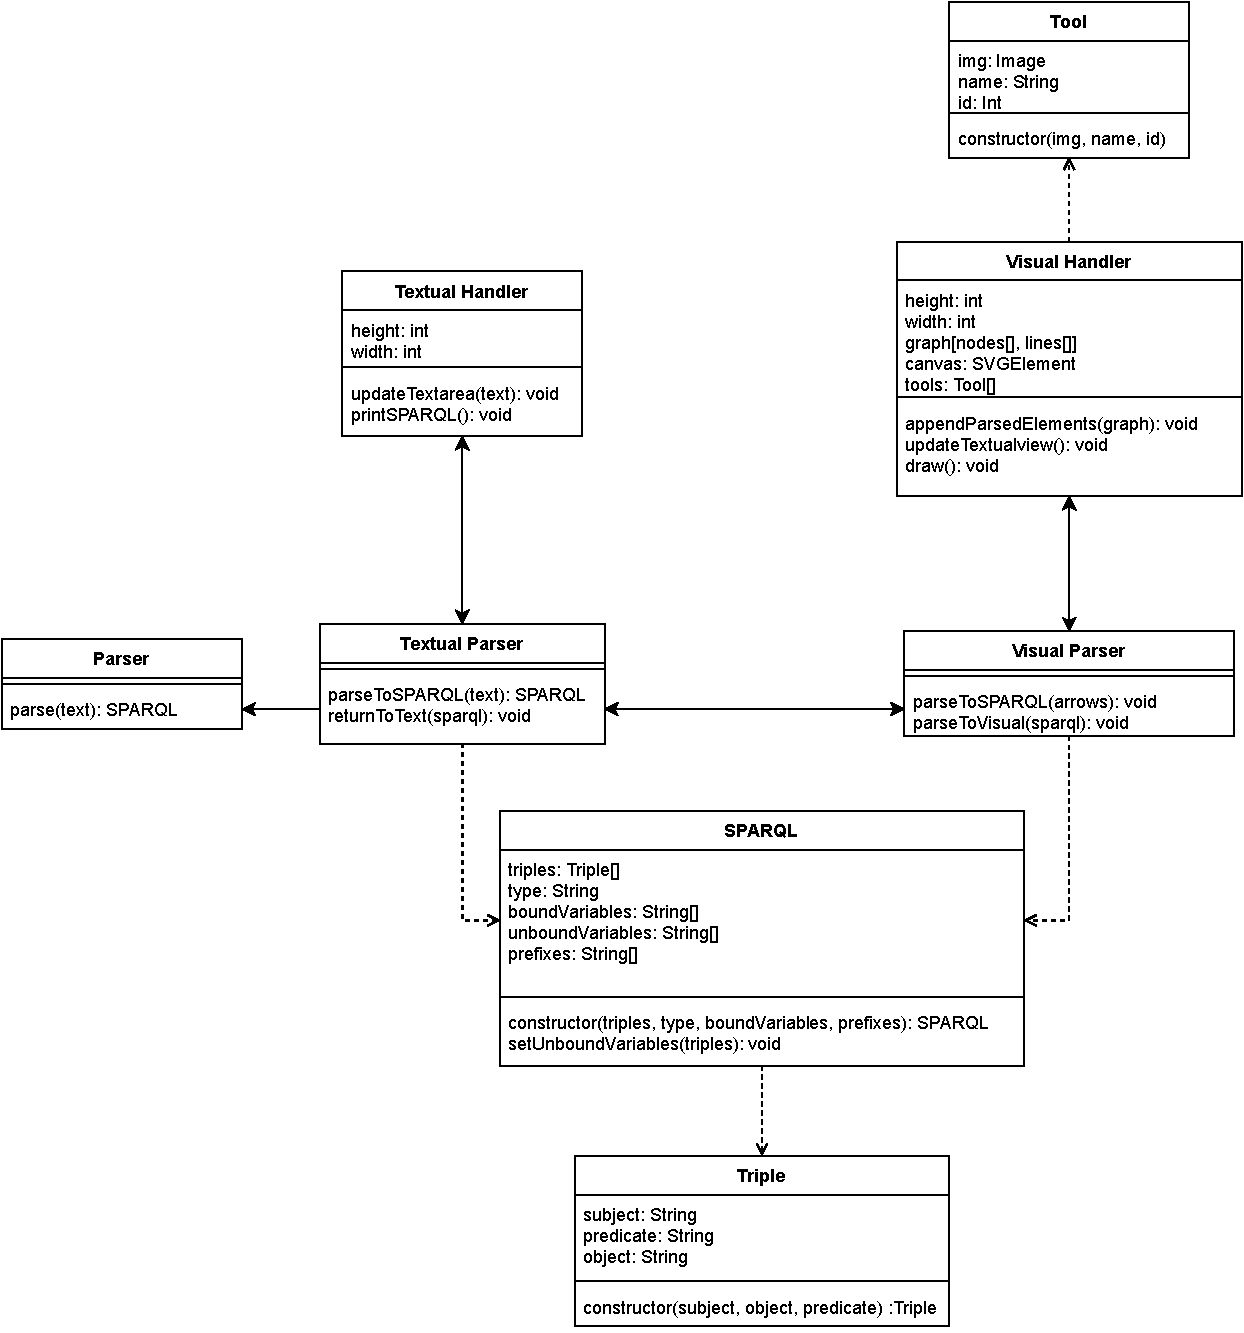
\includegraphics[angle=90,origin=c,width=1.3\textwidth]{figures/2nd_iteration_design.pdf}
    \caption{Caption}
    \label{fig:my_label}
\end{figure}

The way the design changed from the first to the second iteration is the removal of the nodes and arrows objects, as they are no longer needed since they are already being featured in D3.js. This also meant changing from an array of nodes and an array of arrows to a single multi dimensional array. The only thing added during this process has been the parser class
\section{Implementation}
\subsection{Textual Implementation}
The implementation of the textual parser was quite different from the previous work as it now relied on grammar instead of actual JS code. An example of the difference can be seen in figure \ref{fig:pegjs} below:
\begin{figure}[H]
    \centering
    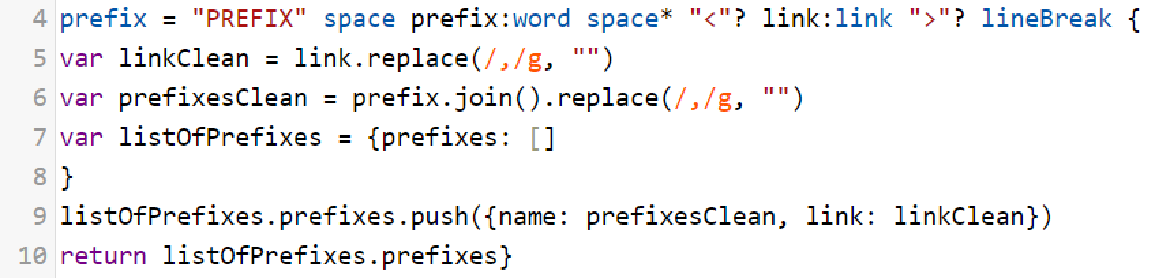
\includegraphics[width=1\textwidth]{figures/pegjs.pdf}
    \caption{Picture of prefix code for parser}
    \label{fig:pegjs}
\end{figure}
Figure \ref{fig:pegjs} also highlights the unforeseen issue we had with the PEG.js parser. The parser returns char arrays instead of strings leading to the strange join and replace functions seen.

\bigskip
The way a parser like this works is by giving it some kind of grammar it can read through and some text. It will then return different objects from the text depending on the grammar. The way this particular parser works is by defining a set of rules. Looking at the example in figure x.x, a prefix is defined as the word PREFIX in all caps followed by a space, then a word which we give the name prefix, so we can refer back to value later, yet another space with an asterix indicating that there can be between 0 and many spaces, then followed by a “<” with the question mark meaning that it does not have to be there but could be, then a link with the name link, another > with a question mark and lastly a line break. This all leads to us being able to grab the two things we gave names to and return as a prefix object when the parser is called. The parser then uses this grammar to create a massively complicated JavaScript file that is the parser itself and the one that runs in our code but we do not have to ever touch this file as its all auto generated so we can just call the parse function and it runs according to the grammar it was created with.

\bigskip
The error handling also changed a lot during the second iteration as the parser used had inbuilt error handling, so we just had to get the message and location to display it in the error handling box. We wanted to implement some highlight of where the error was to make it easier to pinpoint but since HTML does not natively support highlighting in textareas we had to implement the jQuery library called “highlight textarea” this is a quite simple library that allows you to highlight the text of a textarea by giving it either words to highlight or a range to highlight, since the error handling from the parser already include a range of the error this was the obvious choice see figure \ref{fig:errorhandling}:
\begin{figure}[H]
    \centering
    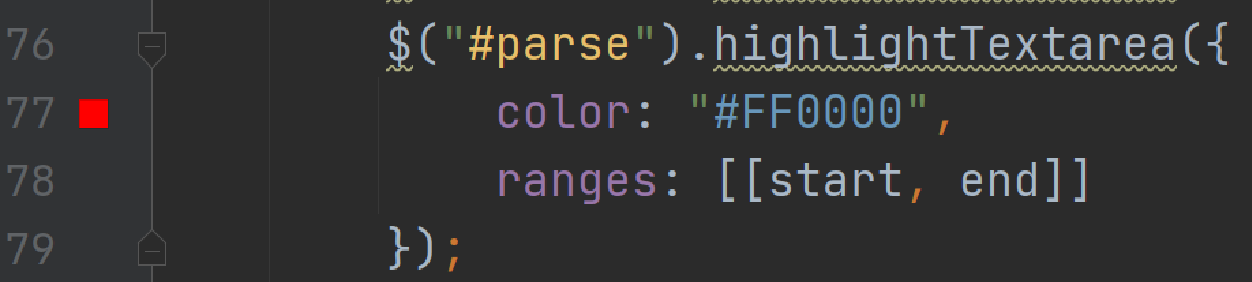
\includegraphics[width=1\textwidth]{figures/errorhandling.pdf}
    \caption{Error handling highlighting}
    \label{fig:errorhandling}
\end{figure}
As can be seen on figure \ref{fig:errorhandling} this is a simple process you just have to give the ID of the textarea and call the highlightTextarea function that takes a colour in this case red to indicate that is an error and the range in this case the start and end of our error.

\subsection{Visual Implementation}
The second iteration led to the implementation of the library D3.js and a couple of new functionalities for the visualisation, see figure \ref{second-iteration-ui}. When implementing d3, the two classes, Node and Arrow, could be removed from the application. The visualisation is now stored in a graph variable containing both nodes and lines, figure \ref{graph}.

\begin{figure}[H]
    \centering
    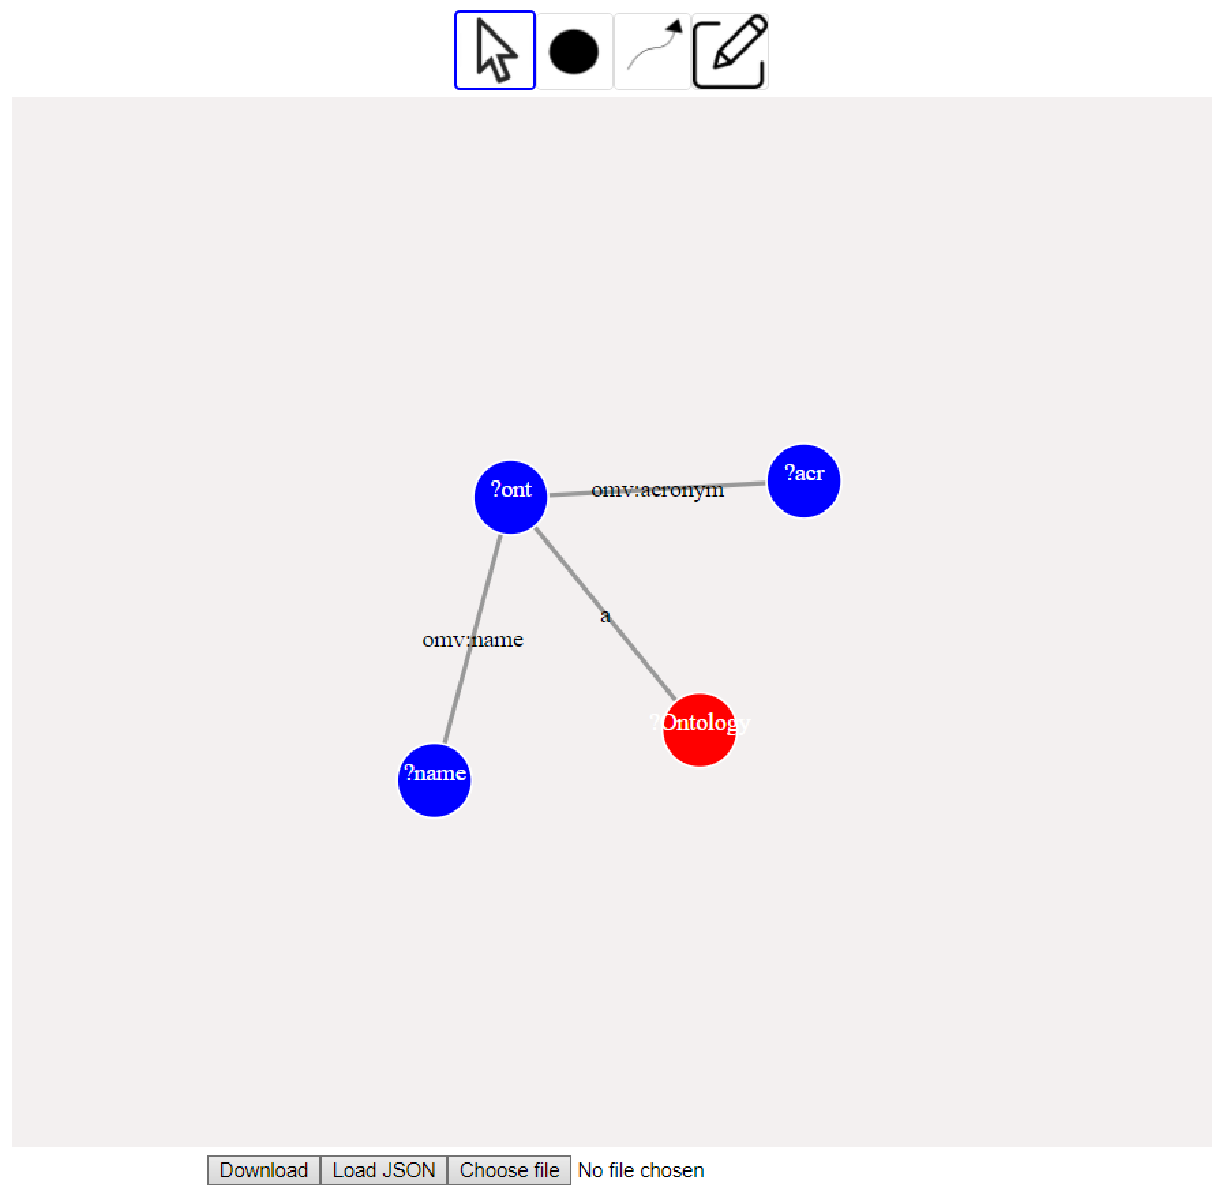
\includegraphics[width=1\textwidth]{figures/second-iteration-ui.pdf}
    \caption{Visual part in the second iteration}
    \label{fig:second-iteration-ui}
\end{figure}

\begin{figure}[H]
    \centering
    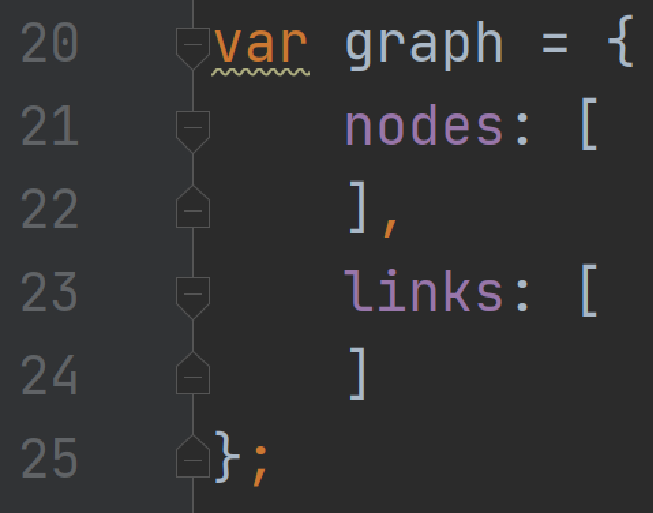
\includegraphics[width=0.5\textwidth]{figures/picture-graph.pdf}
    \caption{The graph variable storing the visualisation}
    \label{fig:graph}
\end{figure}

With the implementation of d3.js, a new version of the force directed graph has been implemented, see figure \ref{fig:forceimplementation}. The written code for the force simulation is significantly shorter than the one implemented in the first iteration, and the second implementation has noticeably more options. As seen on lines 271-274, different attributes of the simulation have been set. These attributes can help push the visualisation toward the centre of the canvas, add collision between the nodes so that they do not overlap, and add a charge to all nodes to push them away from each other. This force simulation is also a part of a bigger draw method, which can easily be called when wanting to update the visualisation. This makes for significantly easier implementation when wanting to add new SVG elements to visualisation. All required of the developer is to add a new group to the draw method, see figure \ref{fig:addednode}. Here the code resembles normal SVG implementation, with the addition of the d3 drag module, line 310-311. This module gives the visualisation the required methods to become more dynamic and draggable by the user.

\begin{figure}[H]
    \centering
    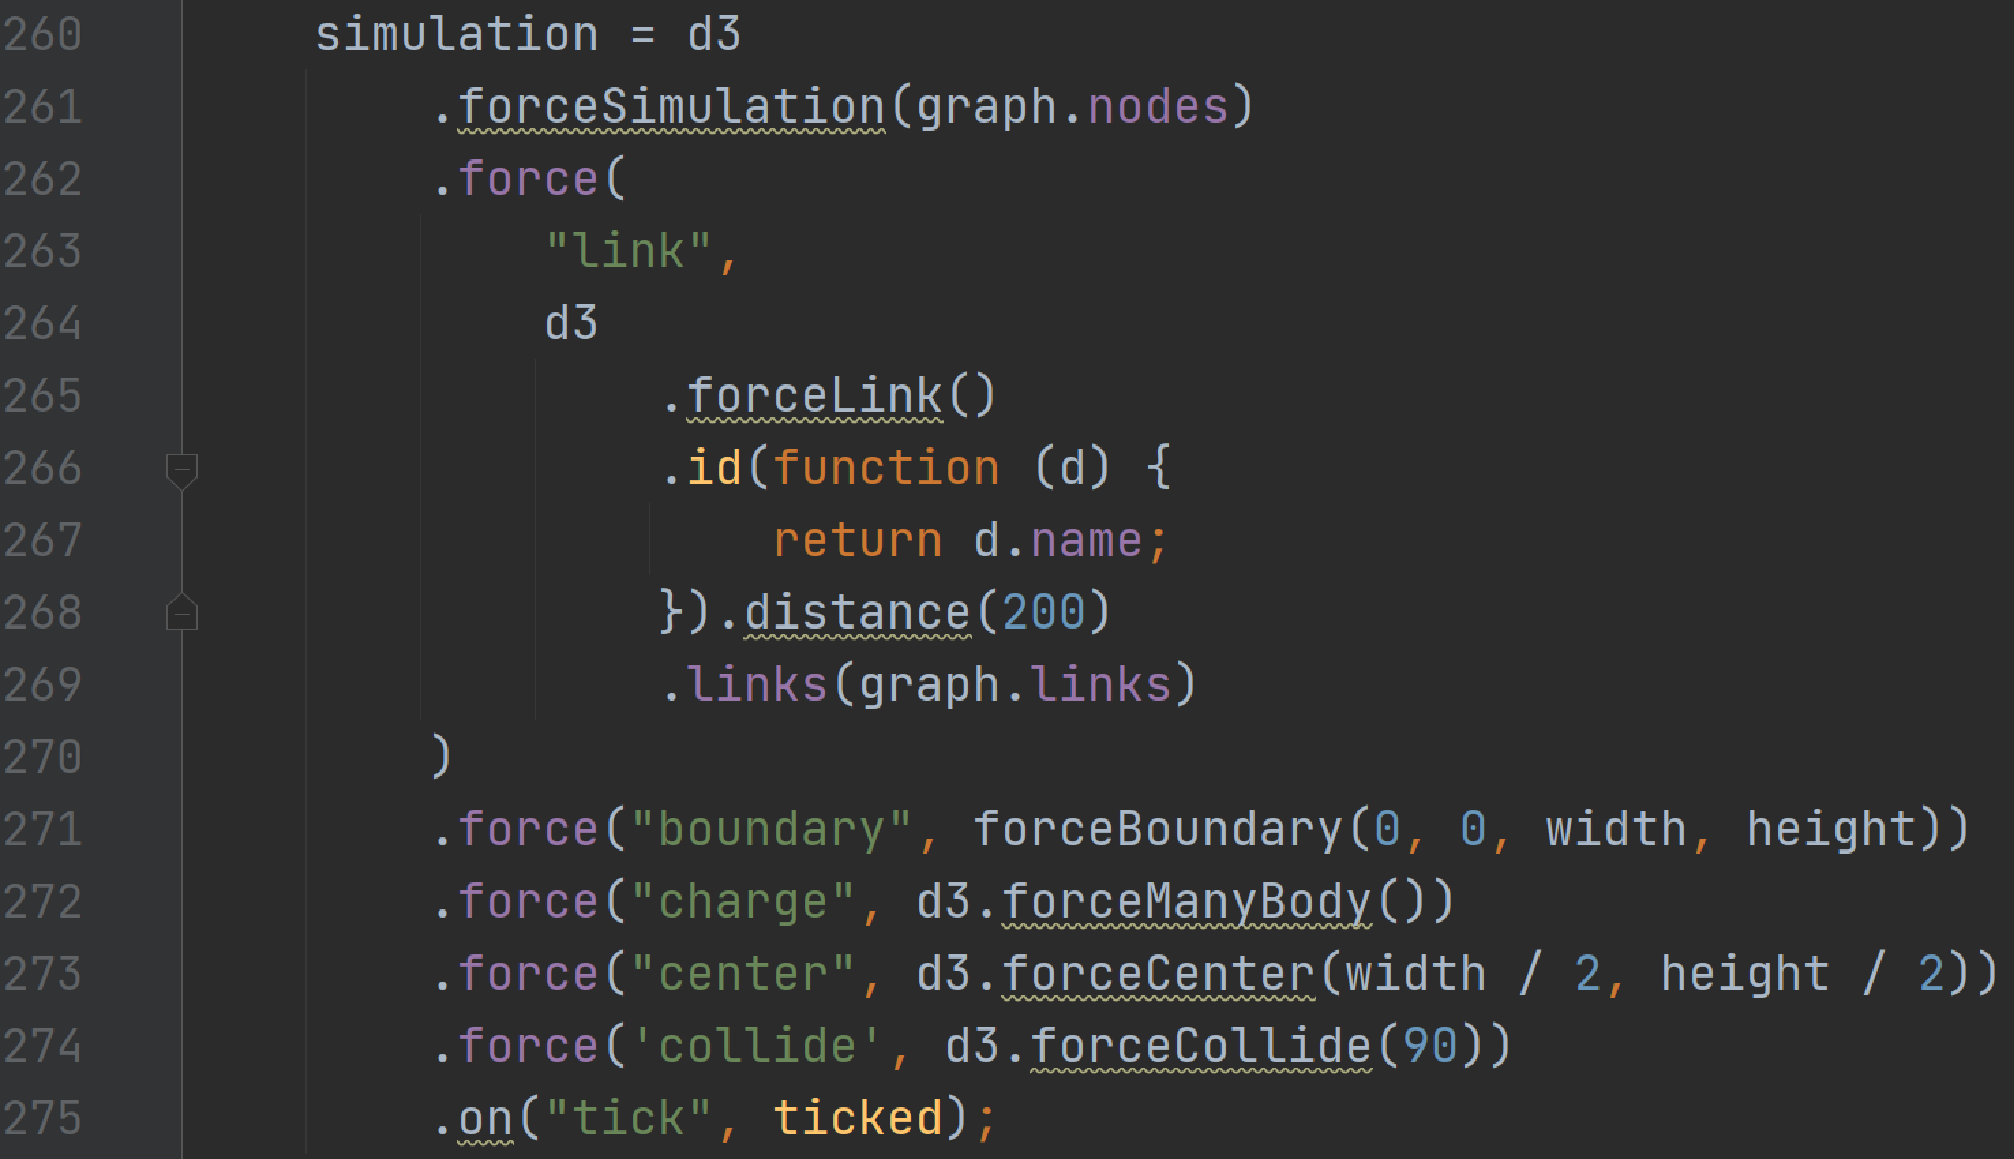
\includegraphics[width=1\textwidth]{figures/force-implementation.pdf}
    \caption{Force implementation with D3.js}
    \label{fig:forceimplementation}
\end{figure}

\begin{figure}[H]
    \centering
    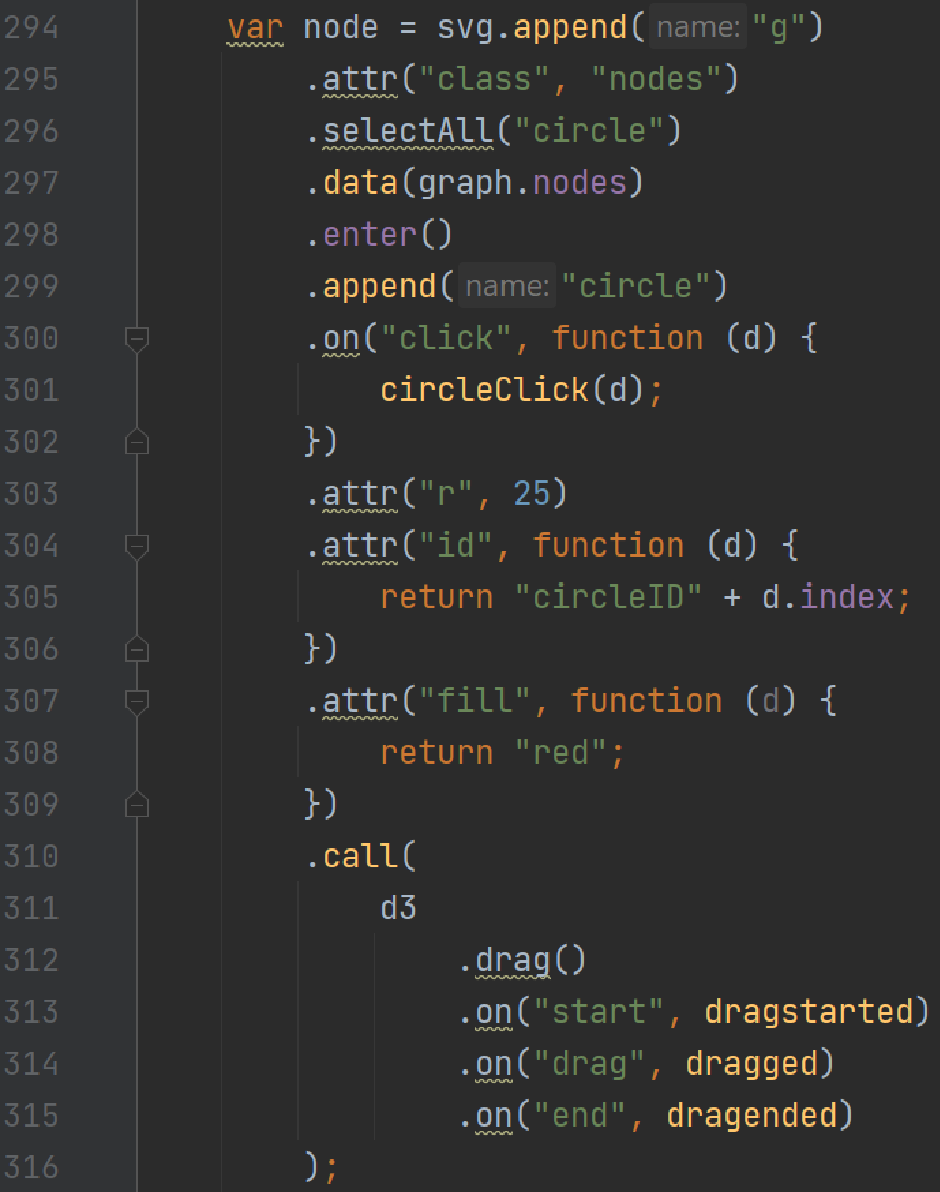
\includegraphics[width=0.8\textwidth]{figures/added-node.pdf}
    \caption{Added node}
    \label{fig:addednode}
\end{figure}

Some of the requirements implemented into this iteration was the ability to download and load the visualisation, see figure \ref{fig:second-iteration-ui}. The group discussed which file format the downloaded file should be, and it ended with a choice of JSON. While JSON does not offer the possibility to view the visualisation as an image, it has easy implementation when converting from the graph variable seen in figure \ref{fig:graph}. JSON also allowed for a simple implementation when uploading which perhaps would have been much more difficult with a file type like JPEG or PNG.
\\
Lastly, a new tool has been added, figure \ref{fig:second-iteration-ui}. The added tool fills the requirements of editing the nodes and arrows. The tool opens the same popup as the creation tools but this time it inputs the selected elements information. In figure \ref{fig:edittool} the edit tool can be seen used on a bounded node called “?name”.

\begin{figure}[H]
    \centering
    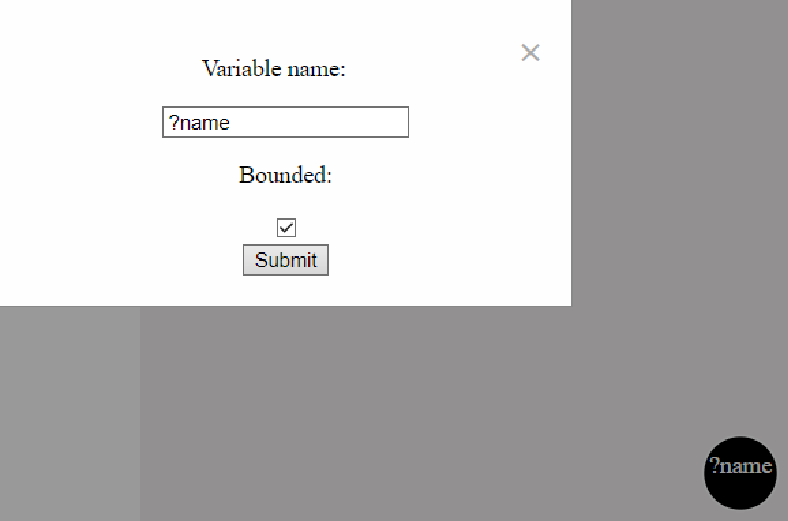
\includegraphics[width=1\textwidth]{figures/edit-tool.pdf}
    \caption{The edit tool in action}
    \label{fig:edittool}
\end{figure}

\section{Testing}
\begin{figure}[H]
    \centering
    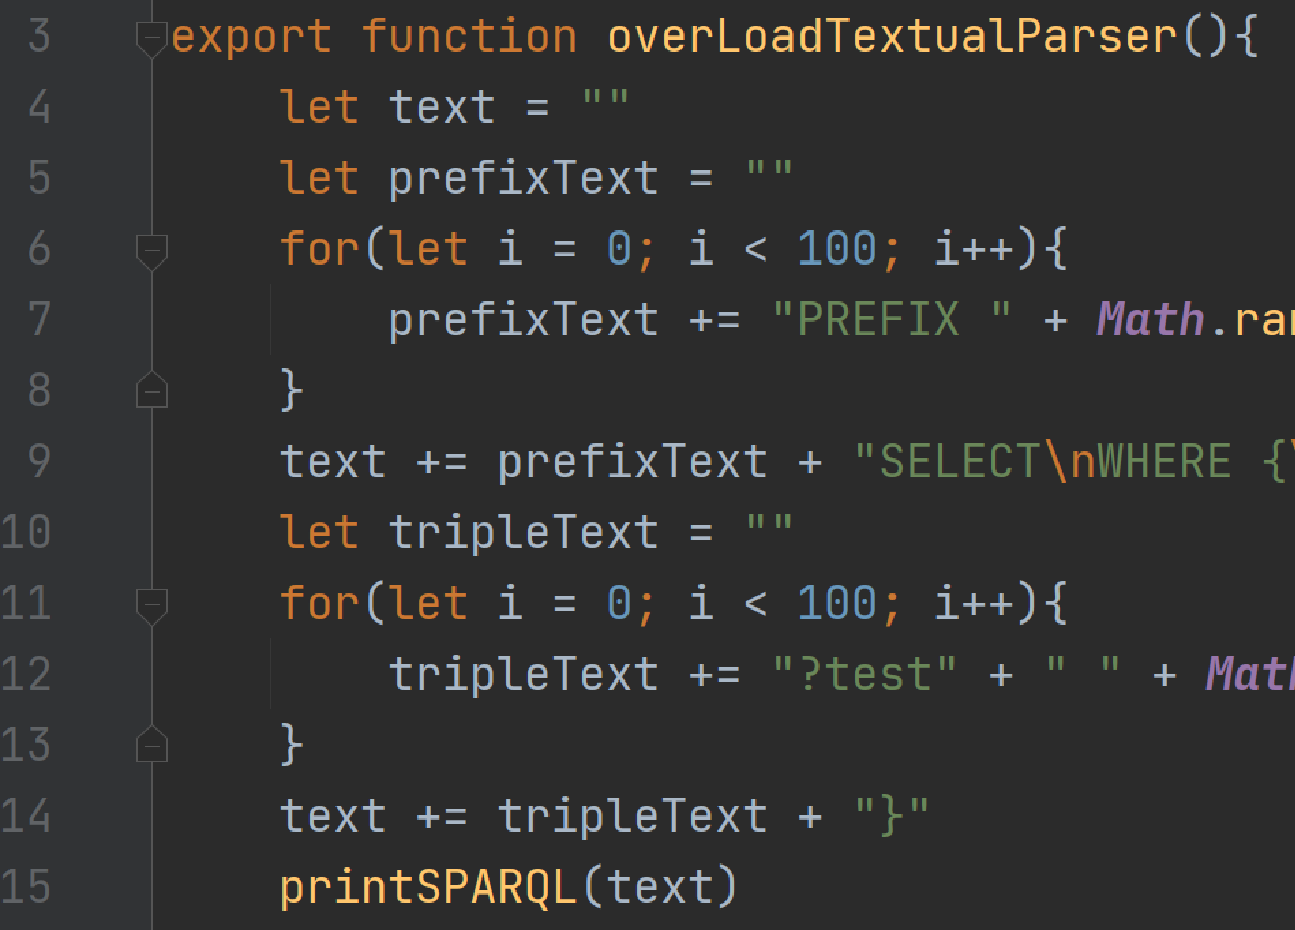
\includegraphics[width=1\textwidth]{figures/overloadgeneration.pdf}
    \caption{Function for overloading both the visual and textual element}
    \label{fig:overload}
\end{figure}
Figure \ref{fig:overload} is a showcase of a function that creates 100 prefixes and 100 triples. This is done to create such a big query that we will never expect a user to input this much data, and can be used as an absolute worst case scenario. The figure \ref{fig:time-forloop} shows the way we went about getting time data and how we ran the test. It's as simple as running the test 100 times and logging when the function started and when the function ended.
\begin{figure}[H]
    \centering
    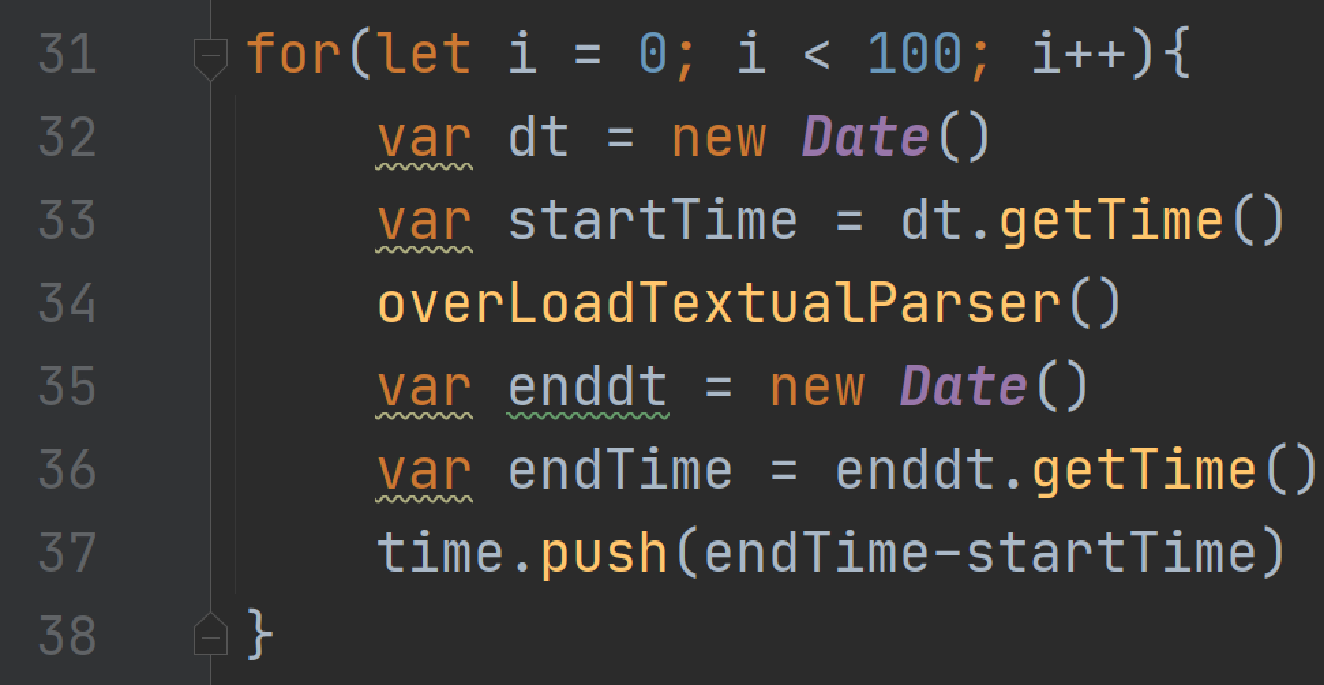
\includegraphics[width=1\textwidth]{figures/time-forloop.pdf}
    \caption{For loop to get the time from start to finish of the overload function}
    \label{fig:time-forloop}
\end{figure}
Figure \ref{fig:array-15} shows the time in milliseconds for the first 15 runs and as can be it is all done within 100ms which was the goal for our performance. 
\begin{figure}[H]
    \centering
    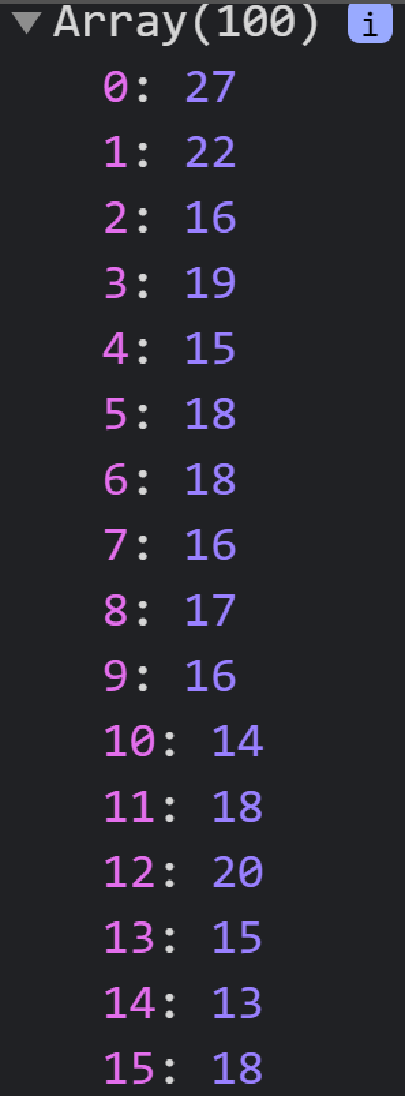
\includegraphics[width=0.2\textwidth]{figures/array-15.pdf}
    \caption{Array showcasing the first 15 times}
    \label{fig:array-15}
\end{figure}
Figure \ref{fig:bad-visual} shows how the visual element handles it and as can be seen it gets quite overloaded and can’t figure where to place things this is in part due to the query being 100 different pairs of nodes being showcased meaning there is simply not enough space on the canvas size chosen, however this is not a big issue as this is way more than a realistic query would like.
\begin{figure}[H]
    \centering
    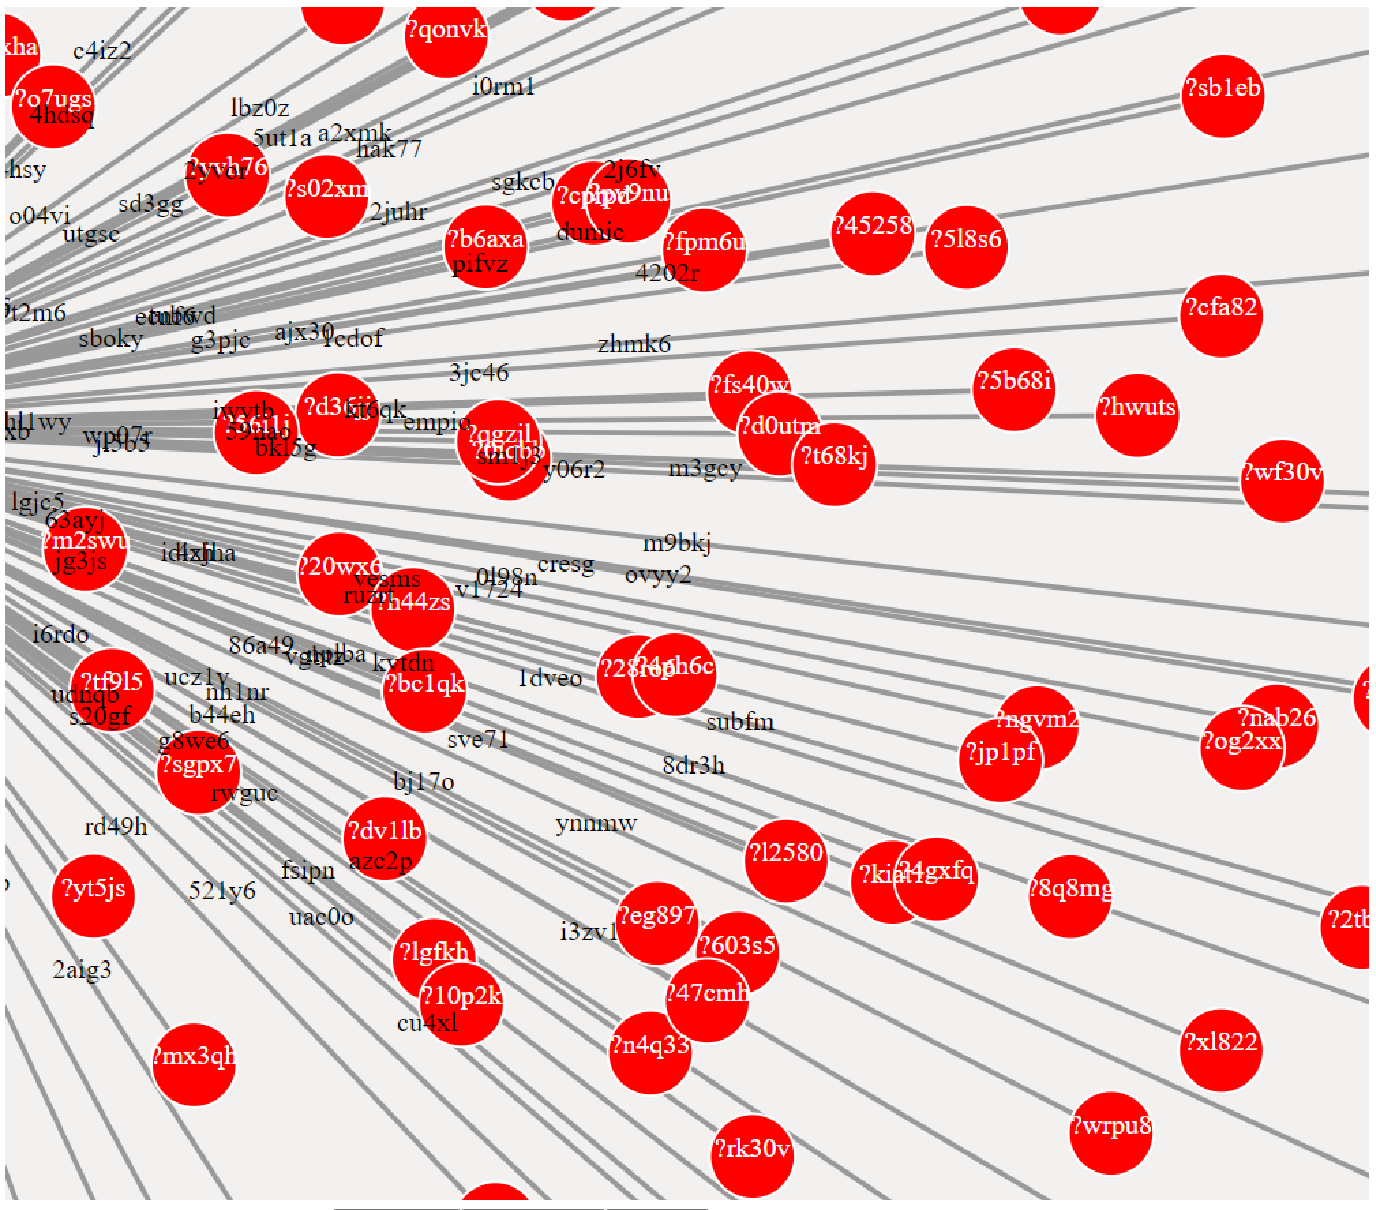
\includegraphics[width=1\textwidth]{figures/bad-visual.pdf}
    \caption{The visual element being under stress}
    \label{fig:bad-visual}
\end{figure}



\section{Evaluation}
\label{chap:second-eval}
When it comes to the textual part of the second iteration, it was a difficult task at hand since we had no experience working with any kind of parser technology. This led to a lot of time spend in the online editor of the parser trying to figure out how does it work and how do we make sure it can handle everything we want, this meant a lot of changes in the grammar along the way and many small bug fixes each taking up anywhere from 1min to multiple hours trying to solve. We also tried to implement some continuous updating, but sadly we could not figure out how to make any of it not annoying when writing the query, as there were some issues with HTML textareas that when you update it unfocuses the textarea meaning the cursor gets put back at the start. Luckily, we managed to fix this issue by a workaround, this just led to the issue of highlighting or error messages getting in the way when trying to type as we figured obviously while typing you do not expect the half-finished work to be error free and therefore, we landed on the click of a button or manually unfocusing the textarea was the best solution. We wanted to implement a way to highlight variables in the query like seen in the “NITELIGHT EXAMPLE'' and figured we would use the same highlight library as before, unfortunately this is library does not support dynamic updates of the code meaning we would write a function for each number of potential variables, we figured this was a solution that scaled so badly that we scrapped the idea.

\bigskip
The visual implementation for the second iteration handled a few requirements not completed in the 1st iteration. While some of those requirements were functional, the focus of this iteration has been with the non-functional requirements. This meant that with the implementation of the library d3.js, there has been significant improvements to the visualisation part. With d3s already implemented force simulation, the force directed graph from the 1st generation has become noticeably smoother and more appealing to look at. D3.js also helped give new functionality by making the nodes draggable. Lastly, d3 has been the codebase more friendly towards further development.
\bigskip
There was not a lot of new functionality for the user in the second iteration, and while this may seem regrettable, there are still significant improvements to the application. The codebase has been significantly improved, making it easier to continue development in later stages, and the already existing functionality has also improved notably, making it a more appealing program. The application is now completely ready for a potential 3rd iteration, which would be an appreciably easier iteration. A potential 3rd iteration would come with a huge functionality boost by simply adding to the already existing library implementations. Especially the parser would see easy implementation as new rules can be added to the grammar file to implement new functionality.

\chapter{Future work}
\label{chap:future-work}

\section{Short term goals}
The most important task for a future improvement would be the implementation of more SPARQL functionality as the second iteration did not add much in this area. The most important functionality to add within the short term would be the UNION and FILTER functions as these work across any query type possible. The last of the requirements that has something to do with functionality of SPARQL is the addition of the DESCRIBE, ASK and CONSTRUCT types. All these would be rather simple to implement now that the code base is supported by external libraries. Going about implementing the additional types could be done in much the same way as the SELECT type, with the biggest challenge being how to effectively visualise them to the user. 

\subsection{Visual}
\subsubsection{New SPARQL functionality}
With the implementation of D3.js, the question of implementing new SPARQL functionality, does not relate to how implement, but rather how the implementation would look. As an example, take the example of the union functionality. Union works by combining two variables\cite{UNIONWiki}. This could perhaps be shown visually with a new type of arrow, a circle around the two nodes, or something entirely else. With the current version of the application, neither of these solutions would be awfully hard to implement, but it must not be confusing for the user. With new functionality there is an increased risk that the visualisation would become chaotic and impossible to navigate. A visualised solution for this must therefore be found before implementing any new features.

\subsubsection{Additional requirements}
A couple of other requirements are still yet to be implemented or improved. One of these requirements is the synchronous highlighting of nodes and text view. A simple change of colour attributes on the nodes would be all that was needed for the visual implementation. Changing the colour of the nodes is something the application already works with, which can be seen when selecting a node, as it changes colour to black. A possible update to the SPARQL class could however be necessary to store the colour of the variables, so that it would be consistent across the application. Highlighting of bound and unbound variables in the textual element was something that was tried and failed, but it was deemed as highly beneficial for the project. The solution here would be to write a custom jQuery library that can handle dynamic updating of highlights throughout.\\
A requirement that needs improvement is the downloading of the visualisation. In the current version, the visualisation is downloadable as a JSON file. While this helped with uploading the visualisation again, a JSON file is not as readable or useful for some as perhaps an image would be. For a potential third iteration, an implementation which also converts d3 to PNG or JPEG is preferred\cite{D3toImage}.\\
Non-functional work for a third iteration could be the addition of an example query on the page, and the resizing of nodes, which do not fit for longer variable names. An example query could help new users significantly, as a direct reference or example is easy to access. A reference to the SPARQL documentation by W3 is also possible\cite{W3Documentation}.

\subsection{Textual}
\subsubsection{Automatic updating}
Automatic updating of the textual view has been tried and failed as explained in chapter \ref{chap:second-eval}. This is still something the project would benefit from greatly and it is therefore worth trying to implement in the short term. A different approach could be to split up the error handling so highlighting only occurs when you press a button. This could be necessary as the highlighting trailing your unfinished query can get quite annoying. There was also an issue of the cursor resetting to the start of the textarea, with a jQuery library this might have an avoidable issue.

\section{Long term goals}
The long-term goals are less likely to ever be implemented and are sometimes also a bit out of the scope of the project. The goals include:
\begin{itemize}
    \item Hooking up to an RDF database
    \item HTML and CSS visual updates
    \item D3 module loading
    \item Different parser implementation
    \item Caching
    \item Implementing a test framework
    \item Autocompletion for the query
    \item Further implementation of SPARQL functions
\end{itemize}
\\
Regarding the first of these goals, the hooking up to an RDF database can certainly be seen as out of the project scope. However, as the group has experienced first-hand, when learning about SPARQL, it can be nice to be able to get a result from your SPARQL query. This helps the understanding of what is returned by a query, or what a query does in general. \\
While the group is happy with the current D3 and parser implementation, possible upgrades can still be made. With the current version of the application, all modules from D3 are loaded. This creates unnecessary load time and can be improved by only importing the needed modules. Looking at the parser, while the action time is great, other parsers were faster as noted in the analysis of the second iteration (chapter \ref{chap:second-analysis}). The group chose PEG.js due to its appreciably easier implementation, and it is therefore a question of whether it is worth it to switch. In its current state, the group does not think it is necessary, but perhaps with an increase in rules, the difference between parsers becomes more apparent. \\
The group also discussed adding a testing framework. A testing framework could help ensure the code is running as expected without bugs, but with the few features in its current version, it did not seem required. A framework that did look interesting to implement was the discovered Jest, which is widely popular amongst JS developers\cite{Jest}. \\
An additional nice to have feature is a caching system. In its current form, the visualisation and written query would be nulled when reloading or experiencing crashes to the system. This would have a noticeable impact when dealing with bigger queries, and it could discourage the use of the system.

\subsection{Visual}
\subsubsection{Performance}
At the moment of writing, it is believed that the performance of the visualisation is greatly affected by the size of the canvas. This is due to the force simulation wanting to settle, which is impossible with too many nodes in too little space. Therefore, a possible solution to this problem could be to make the canvas larger, or the nodes smaller, and then implement panning and zooming so that the user experience is not affected negatively. D3 also has modules for zooming and panning\cite{d3zoom}. How this would affect a possible image download is still unknown at this point, but the guess is that it would make it a lot harder to see what is going on with the nodes being smaller compared to the canvas.
\subsection{Textual}
The final long-term issue is autocompletion which can be used in two instances. One would be the autocompletion of common RDF prefixes i.e. typing “PREFIX foaf:” would yield “PREFIX foaf: http://xmlns.com/foaf/0.1/”. The second instance could be in the sense of autocompleting SPARQL query entries like most IDEs have for programming languages. An example could be typing “?na”, which would allow for the autocompletion to “?name” if that was a variable in the system. 

\chapter{Conclusion}
\label{chap:conclusion}

Overall our project was a success.


\chapter{Project Evaluation}
\label{chap:project-evaluation}

\subsection{COVID-19}
Due to COVID-19 we could not carry out in person supervisor meetings, which could have had an impact on the feedback between the group and the supervisor. The group does however think that the online meetings were utilised to its full capabilities, and communication was still possible, even outside of the meetings. COVID also had an impact on the ability to have people test our software in person, which lead to us having worse feedback than was optimal. As our application has great focus on the user, it would have been ideal if a user test session was possible. Lastly, being stuck at home also had an effect on the progress of the project, as scheduling and maintaining meetings between the group proved difficult.
\subsection{Development}
During this project the group used an iterative development model. Overall the development process was effective but unstructured, and a more structured development method could have been useful. This especially comes to mind when considering the size of the project, meaning that it was difficult to manage everything with the lack of tools used throughout. Potential tools and methods that could have been used to help structure is the kanban board, taking elements from Scrum such as the daily meetings, or a more structured development method like AUP or RUP.\\
Throughout the project there were multiple times where the group was distracted and busy with other projects and courses due this semester. This meant that it was not possible to devote our full time to this project and this lead to some weeks were little to none progress were made.\\
Lastly, when working with new subjects such as SPARQL and RDF, there is big reason to do lots of research in the first part of the project. This of course helped us develop a better system, but there were however feelings of being stuck.
\subsection{Product}
Overall the group is satisfied with the product outcome of the project. The product hit all the major requirements we wanted and the few requirements we did not manage were due to unforeseen issues we could not solve in time. The implementation of the product helped us learn a lot about JavaScript development, the RDF and SPARQL connection and how to work in this type of project. The group was not used to work on open ended projects and were not used to work on projects of this size in pairs. For future projects we now also know what is required to work with an unknown subject, and will not be discouraged by the feeling of going nowhere, as we know that progress is slow.

\chapter{User manual}
\section{Install web component}
To install the application simply add the script to your HTML file as shown in figure \ref{fig:install}
\begin{figure}[H]
    \centering
    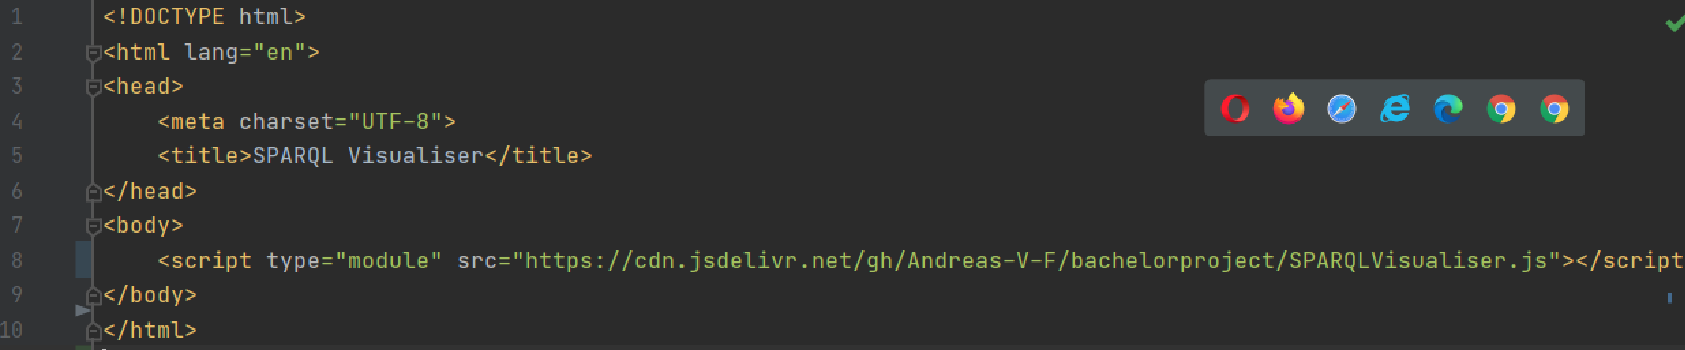
\includegraphics[width=1\textwidth]{figures/install.pdf}
    \caption{Installation of the software}
    \label{fig:install}
\end{figure}
\section{Using the software}
Nodes are draggable by holding the left mouse button down. 
\subsection{Add node}
To add a node to the visualisation click the Add node tool. A popup will be shown, see figure \ref{fig:user-add}. Fill out the name and whether the node should be bounded or not. A bounded variable will be shown as blue while an unbounded variable will be red.

\begin{figure}[H]
    \centering
    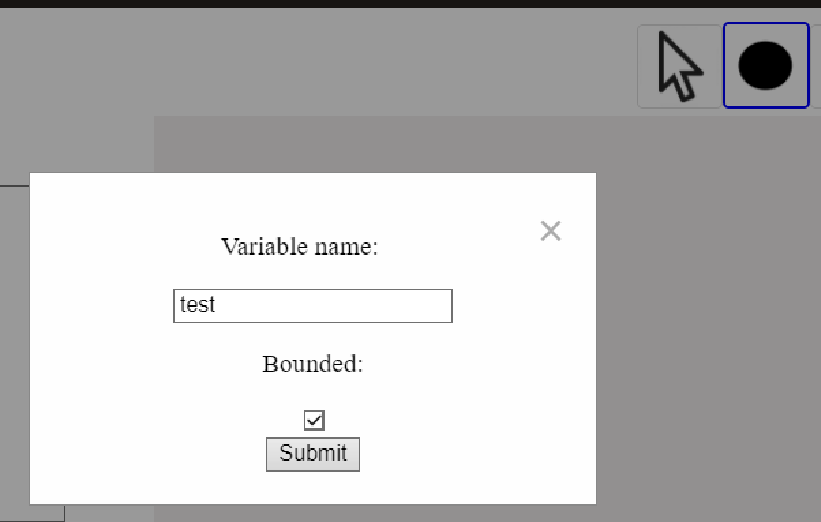
\includegraphics[width=1\textwidth]{figures/add-node-user.pdf}
    \caption{Adding a node}
    \label{fig:user-add}
\end{figure}
\subsection{Draw line}
Select the connect nodes tool. Now click two nodes which are not already connected. Fill out the predicate name, see figure \ref{fig:user-line}. As well as the now added line, you will see an update to the text area in the top left.
\begin{figure}[H]
    \centering
    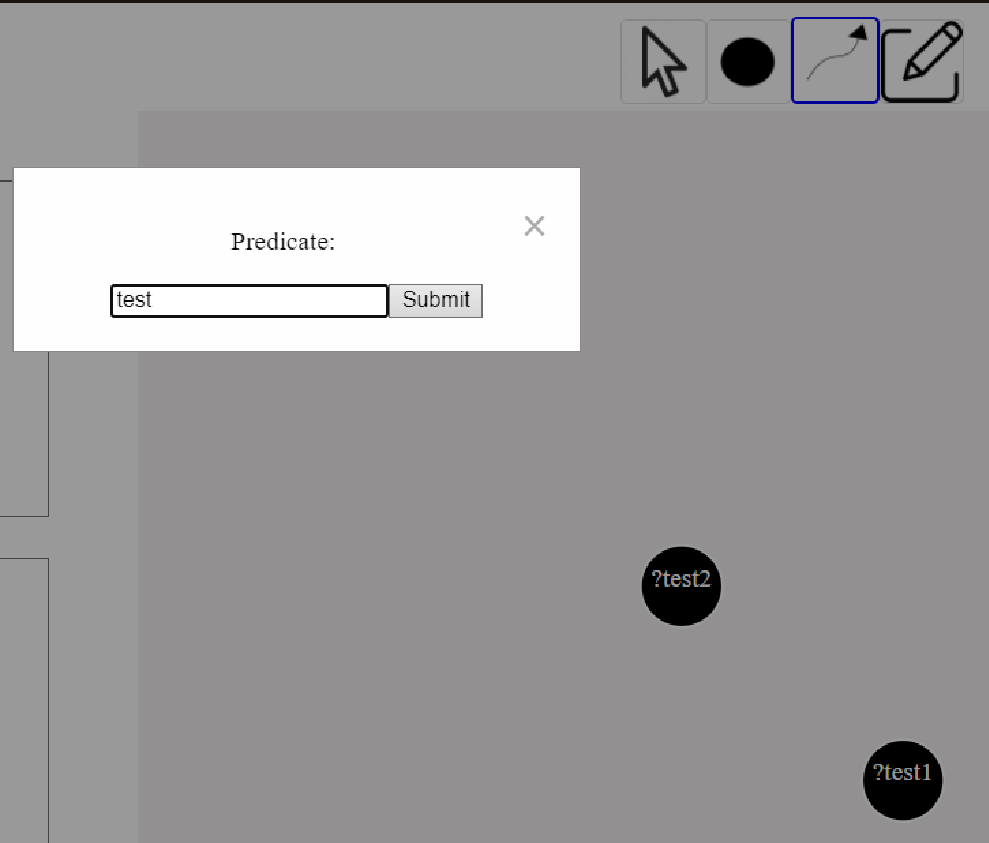
\includegraphics{figures/add-line-user.pdf}
    \caption{Adding a line}
    \label{fig:user-line}
\end{figure}
\subsection{Write query}
Go to the text area in the top left. Fill out a query. Press the run button to run the parser. If your query is insufficient, an error message will show in the text area below, figure \ref{fig:user-write-error}. Use this error message to figure out how to correct your query. On a successful parse, your query will be shown in the visualisation, figure \ref{fig:visual-success}.
\begin{figure}[H]
    \centering
    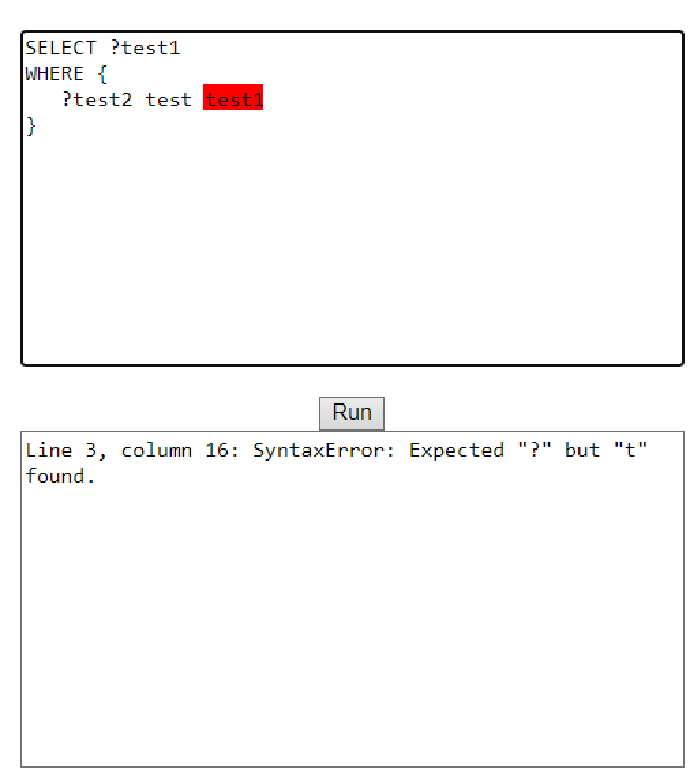
\includegraphics[width=0.6\textwidth]{figures/user-write-error.pdf}
    \caption{Caption}
    \label{fig:user-write-error}
\end{figure}

\begin{figure}[H]
    \centering
    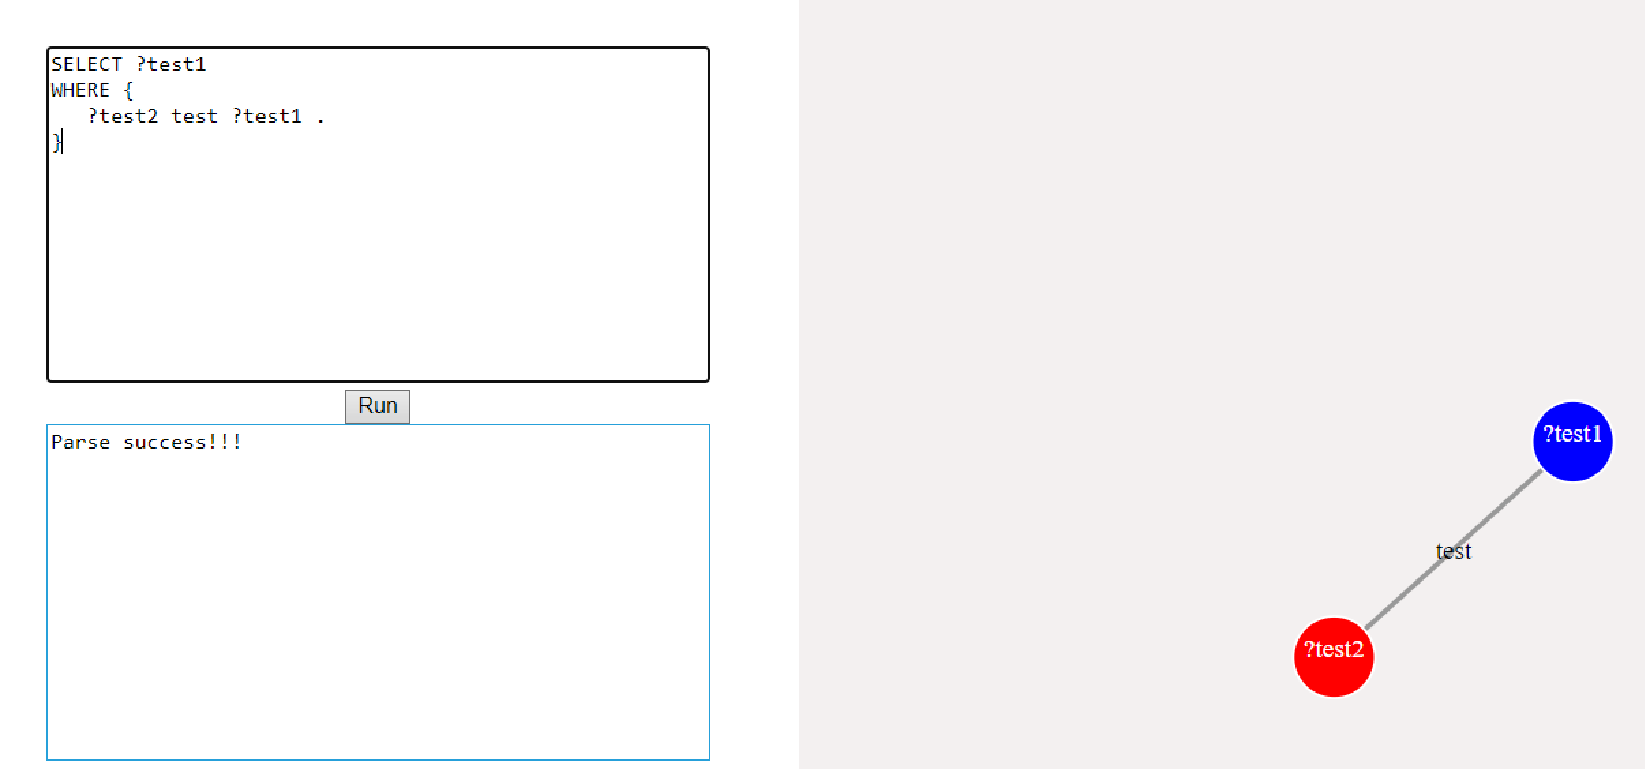
\includegraphics[width=1\textwidth]{figures/visual-query-succ.pdf}
    \caption{Caption}
    \label{fig:visual-success}
\end{figure}

\subsection{Selection}
Click on the select tool. When clicking on either a node or a line, they will be added to the selection. Selected elements are shown as black, figure \ref{fig:user-select}. If you want to delete selected elements, press the delete key on the keyboard.
\begin{figure}[H]
    \centering
    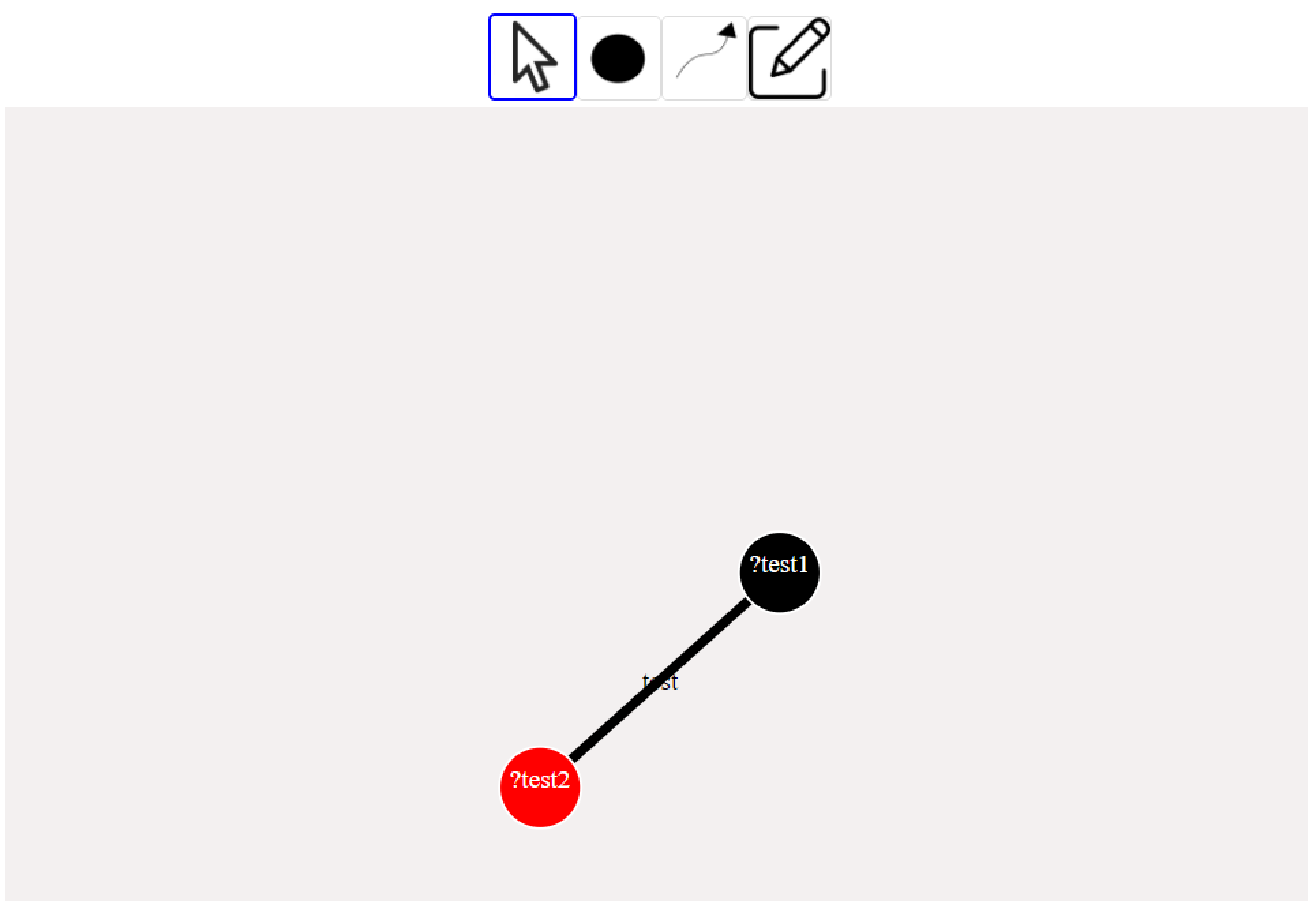
\includegraphics{figures/user-select.pdf}
    \caption{A showcase of }
    \label{fig:user-select}
\end{figure}
\subsection{Editing}
Choose the edit tool. Click either a node or a line. A popup will occur with the selected elements information\ref{fig:user-edit}. Change the information and press submit to edit.
\begin{figure}[H]
    \centering
    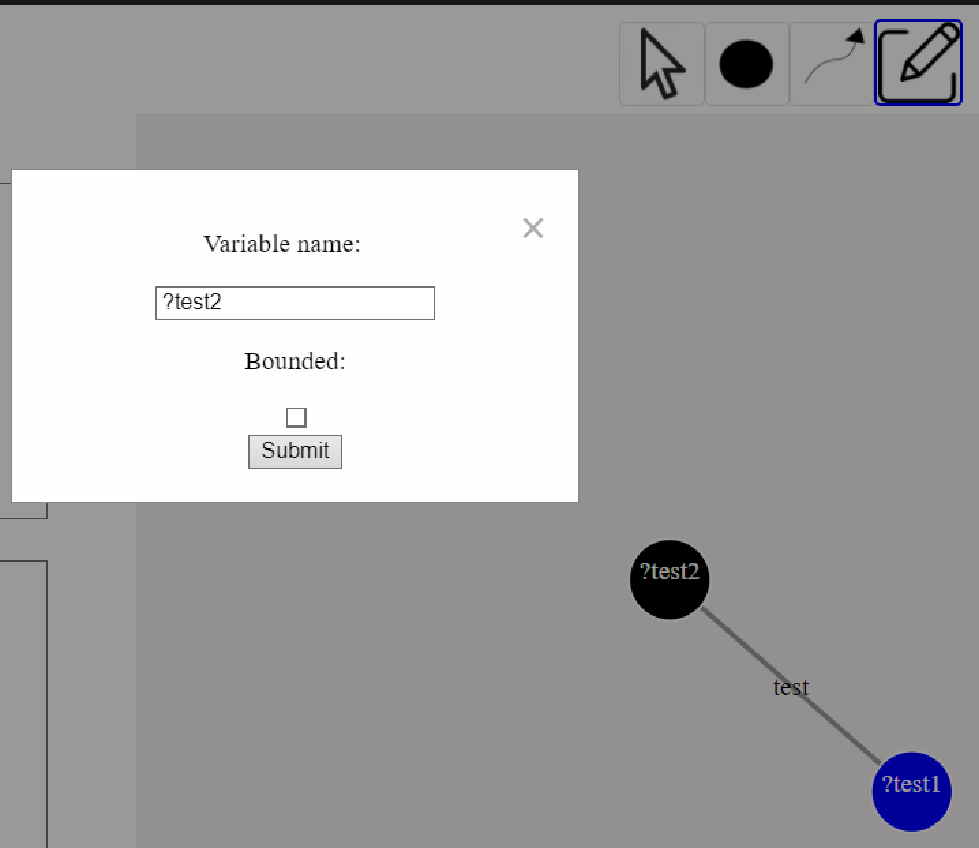
\includegraphics{figures/user-edit.pdf}
    \caption{The edit tool in action}
    \label{fig:user-edit}
\end{figure}
\subsection{Downloading and uploading}
To download the visualisation click the download button. A JSON file will be downloaded to your computer. To load the JSON file, use the choose file button and locate the JSON file. Now click upload. The visualisation and textual area shall be updated to resemble your previously download JSON.

\appendix

\chapter{Appendix}
\label{appendix:api-doc}

We include here the API documentation for our library.


\bibliographystyle{IEEEtran}
\bibliography{mybibliography}

\newpage

\listoffigures

\newpage

\listoftables

\newpage


\end{document}
